% Options for packages loaded elsewhere
\PassOptionsToPackage{unicode}{hyperref}
\PassOptionsToPackage{hyphens}{url}
\PassOptionsToPackage{dvipsnames,svgnames,x11names}{xcolor}
%
\documentclass[
  letterpaper,
  DIV=11,
  numbers=noendperiod]{scrartcl}

\usepackage{amsmath,amssymb}
\usepackage{iftex}
\ifPDFTeX
  \usepackage[T1]{fontenc}
  \usepackage[utf8]{inputenc}
  \usepackage{textcomp} % provide euro and other symbols
\else % if luatex or xetex
  \usepackage{unicode-math}
  \defaultfontfeatures{Scale=MatchLowercase}
  \defaultfontfeatures[\rmfamily]{Ligatures=TeX,Scale=1}
\fi
\usepackage{lmodern}
\ifPDFTeX\else  
    % xetex/luatex font selection
\fi
% Use upquote if available, for straight quotes in verbatim environments
\IfFileExists{upquote.sty}{\usepackage{upquote}}{}
\IfFileExists{microtype.sty}{% use microtype if available
  \usepackage[]{microtype}
  \UseMicrotypeSet[protrusion]{basicmath} % disable protrusion for tt fonts
}{}
\makeatletter
\@ifundefined{KOMAClassName}{% if non-KOMA class
  \IfFileExists{parskip.sty}{%
    \usepackage{parskip}
  }{% else
    \setlength{\parindent}{0pt}
    \setlength{\parskip}{6pt plus 2pt minus 1pt}}
}{% if KOMA class
  \KOMAoptions{parskip=half}}
\makeatother
\usepackage{xcolor}
\setlength{\emergencystretch}{3em} % prevent overfull lines
\setcounter{secnumdepth}{5}
% Make \paragraph and \subparagraph free-standing
\ifx\paragraph\undefined\else
  \let\oldparagraph\paragraph
  \renewcommand{\paragraph}[1]{\oldparagraph{#1}\mbox{}}
\fi
\ifx\subparagraph\undefined\else
  \let\oldsubparagraph\subparagraph
  \renewcommand{\subparagraph}[1]{\oldsubparagraph{#1}\mbox{}}
\fi

\usepackage{color}
\usepackage{fancyvrb}
\newcommand{\VerbBar}{|}
\newcommand{\VERB}{\Verb[commandchars=\\\{\}]}
\DefineVerbatimEnvironment{Highlighting}{Verbatim}{commandchars=\\\{\}}
% Add ',fontsize=\small' for more characters per line
\usepackage{framed}
\definecolor{shadecolor}{RGB}{241,243,245}
\newenvironment{Shaded}{\begin{snugshade}}{\end{snugshade}}
\newcommand{\AlertTok}[1]{\textcolor[rgb]{0.68,0.00,0.00}{#1}}
\newcommand{\AnnotationTok}[1]{\textcolor[rgb]{0.37,0.37,0.37}{#1}}
\newcommand{\AttributeTok}[1]{\textcolor[rgb]{0.40,0.45,0.13}{#1}}
\newcommand{\BaseNTok}[1]{\textcolor[rgb]{0.68,0.00,0.00}{#1}}
\newcommand{\BuiltInTok}[1]{\textcolor[rgb]{0.00,0.23,0.31}{#1}}
\newcommand{\CharTok}[1]{\textcolor[rgb]{0.13,0.47,0.30}{#1}}
\newcommand{\CommentTok}[1]{\textcolor[rgb]{0.37,0.37,0.37}{#1}}
\newcommand{\CommentVarTok}[1]{\textcolor[rgb]{0.37,0.37,0.37}{\textit{#1}}}
\newcommand{\ConstantTok}[1]{\textcolor[rgb]{0.56,0.35,0.01}{#1}}
\newcommand{\ControlFlowTok}[1]{\textcolor[rgb]{0.00,0.23,0.31}{#1}}
\newcommand{\DataTypeTok}[1]{\textcolor[rgb]{0.68,0.00,0.00}{#1}}
\newcommand{\DecValTok}[1]{\textcolor[rgb]{0.68,0.00,0.00}{#1}}
\newcommand{\DocumentationTok}[1]{\textcolor[rgb]{0.37,0.37,0.37}{\textit{#1}}}
\newcommand{\ErrorTok}[1]{\textcolor[rgb]{0.68,0.00,0.00}{#1}}
\newcommand{\ExtensionTok}[1]{\textcolor[rgb]{0.00,0.23,0.31}{#1}}
\newcommand{\FloatTok}[1]{\textcolor[rgb]{0.68,0.00,0.00}{#1}}
\newcommand{\FunctionTok}[1]{\textcolor[rgb]{0.28,0.35,0.67}{#1}}
\newcommand{\ImportTok}[1]{\textcolor[rgb]{0.00,0.46,0.62}{#1}}
\newcommand{\InformationTok}[1]{\textcolor[rgb]{0.37,0.37,0.37}{#1}}
\newcommand{\KeywordTok}[1]{\textcolor[rgb]{0.00,0.23,0.31}{#1}}
\newcommand{\NormalTok}[1]{\textcolor[rgb]{0.00,0.23,0.31}{#1}}
\newcommand{\OperatorTok}[1]{\textcolor[rgb]{0.37,0.37,0.37}{#1}}
\newcommand{\OtherTok}[1]{\textcolor[rgb]{0.00,0.23,0.31}{#1}}
\newcommand{\PreprocessorTok}[1]{\textcolor[rgb]{0.68,0.00,0.00}{#1}}
\newcommand{\RegionMarkerTok}[1]{\textcolor[rgb]{0.00,0.23,0.31}{#1}}
\newcommand{\SpecialCharTok}[1]{\textcolor[rgb]{0.37,0.37,0.37}{#1}}
\newcommand{\SpecialStringTok}[1]{\textcolor[rgb]{0.13,0.47,0.30}{#1}}
\newcommand{\StringTok}[1]{\textcolor[rgb]{0.13,0.47,0.30}{#1}}
\newcommand{\VariableTok}[1]{\textcolor[rgb]{0.07,0.07,0.07}{#1}}
\newcommand{\VerbatimStringTok}[1]{\textcolor[rgb]{0.13,0.47,0.30}{#1}}
\newcommand{\WarningTok}[1]{\textcolor[rgb]{0.37,0.37,0.37}{\textit{#1}}}

\providecommand{\tightlist}{%
  \setlength{\itemsep}{0pt}\setlength{\parskip}{0pt}}\usepackage{longtable,booktabs,array}
\usepackage{calc} % for calculating minipage widths
% Correct order of tables after \paragraph or \subparagraph
\usepackage{etoolbox}
\makeatletter
\patchcmd\longtable{\par}{\if@noskipsec\mbox{}\fi\par}{}{}
\makeatother
% Allow footnotes in longtable head/foot
\IfFileExists{footnotehyper.sty}{\usepackage{footnotehyper}}{\usepackage{footnote}}
\makesavenoteenv{longtable}
\usepackage{graphicx}
\makeatletter
\def\maxwidth{\ifdim\Gin@nat@width>\linewidth\linewidth\else\Gin@nat@width\fi}
\def\maxheight{\ifdim\Gin@nat@height>\textheight\textheight\else\Gin@nat@height\fi}
\makeatother
% Scale images if necessary, so that they will not overflow the page
% margins by default, and it is still possible to overwrite the defaults
% using explicit options in \includegraphics[width, height, ...]{}
\setkeys{Gin}{width=\maxwidth,height=\maxheight,keepaspectratio}
% Set default figure placement to htbp
\makeatletter
\def\fps@figure{htbp}
\makeatother

\KOMAoption{captions}{tableheading}
\makeatletter
\makeatother
\makeatletter
\makeatother
\makeatletter
\@ifpackageloaded{caption}{}{\usepackage{caption}}
\AtBeginDocument{%
\ifdefined\contentsname
  \renewcommand*\contentsname{Table of contents}
\else
  \newcommand\contentsname{Table of contents}
\fi
\ifdefined\listfigurename
  \renewcommand*\listfigurename{List of Figures}
\else
  \newcommand\listfigurename{List of Figures}
\fi
\ifdefined\listtablename
  \renewcommand*\listtablename{List of Tables}
\else
  \newcommand\listtablename{List of Tables}
\fi
\ifdefined\figurename
  \renewcommand*\figurename{Figure}
\else
  \newcommand\figurename{Figure}
\fi
\ifdefined\tablename
  \renewcommand*\tablename{Table}
\else
  \newcommand\tablename{Table}
\fi
}
\@ifpackageloaded{float}{}{\usepackage{float}}
\floatstyle{ruled}
\@ifundefined{c@chapter}{\newfloat{codelisting}{h}{lop}}{\newfloat{codelisting}{h}{lop}[chapter]}
\floatname{codelisting}{Listing}
\newcommand*\listoflistings{\listof{codelisting}{List of Listings}}
\makeatother
\makeatletter
\@ifpackageloaded{caption}{}{\usepackage{caption}}
\@ifpackageloaded{subcaption}{}{\usepackage{subcaption}}
\makeatother
\makeatletter
\@ifpackageloaded{tcolorbox}{}{\usepackage[skins,breakable]{tcolorbox}}
\makeatother
\makeatletter
\@ifundefined{shadecolor}{\definecolor{shadecolor}{rgb}{.97, .97, .97}}
\makeatother
\makeatletter
\makeatother
\makeatletter
\makeatother
\ifLuaTeX
  \usepackage{selnolig}  % disable illegal ligatures
\fi
\IfFileExists{bookmark.sty}{\usepackage{bookmark}}{\usepackage{hyperref}}
\IfFileExists{xurl.sty}{\usepackage{xurl}}{} % add URL line breaks if available
\urlstyle{same} % disable monospaced font for URLs
\hypersetup{
  pdftitle={Assessing Best Fit Model and factors that Contribute to Prediction Of Heart Attack Risk in Global Populations},
  pdfauthor={Aaron Yang, Modupeola Fagbenro, Bharath Genji Mohana Ranga, Kundana Chowdary Cherukuri},
  colorlinks=true,
  linkcolor={blue},
  filecolor={Maroon},
  citecolor={Blue},
  urlcolor={Blue},
  pdfcreator={LaTeX via pandoc}}

\title{Assessing Best Fit Model and factors that Contribute to
Prediction Of Heart Attack Risk in Global Populations}
\author{Aaron Yang, Modupeola Fagbenro, Bharath Genji Mohana Ranga,
Kundana Chowdary Cherukuri}
\date{}

\begin{document}
\maketitle
\ifdefined\Shaded\renewenvironment{Shaded}{\begin{tcolorbox}[interior hidden, enhanced, borderline west={3pt}{0pt}{shadecolor}, frame hidden, sharp corners, breakable, boxrule=0pt]}{\end{tcolorbox}}\fi

\renewcommand*\contentsname{Table of contents}
{
\hypersetup{linkcolor=}
\setcounter{tocdepth}{3}
\tableofcontents
}
\hypertarget{abstract}{%
\section{ABSTRACT}\label{abstract}}

This study delves into the dynamics of electric vehicle (EV) adoption
across different regions in the United States, highlighting regional
disparities and EV growth trends. The study investigates factors
influencing adoption rates, such as state policies, economic incentives,
and infrastructure development, using a large dataset. The goal is to
identify patterns and potential areas for policy intervention by better
understanding the impact of regional characteristics on EV popularity.
This analysis is critical for automotive industry stakeholders,
policymakers, and environmental advocates, as it provides insight into
the future trajectory of sustainable transportation in America.

\hypertarget{introduction}{%
\section{Introduction}\label{introduction}}

The transition to electric vehicles (EVs) is a critical component of the
global transition to sustainability, particularly in the context of the
United States, where transportation contributes significantly to carbon
emissions. The purpose of this study is to dissect the complexities of
EV adoption across various American regions, highlighting the
disparities and underlying factors that influence this trend. The
study's foundation is a large dataset that reflects the multifaceted
nature of EV proliferation, including variables like vehicle types,
regional distributions, and chronological adoption trends.

The dataset's richness allows for in-depth exploration of state-by-state
vehicle counts, county-level data, and vehicle primary use categories.
This study not only highlights the current state of EV adoption, but
also delves into the economic, policy-driven, and infrastructure factors
driving this movement. This type of analysis is critical for
policymakers, industry stakeholders, and environmentalists because it
provides actionable insights to encourage EV integration.

In essence, this study not only maps the current landscape of EV
adoption in the United States, but it also serves as a strategic guide
for navigating the challenges and capitalising on the opportunities in
this domain. It exemplifies the potential of sustainable transport and
the critical role of informed decision-making in meeting environmental
targets.

\hypertarget{summary-of-the-dataset}{%
\section{Summary of the Dataset}\label{summary-of-the-dataset}}

This study's dataset includes extensive records of electric vehicle (EV)
adoption across the United States. It contains information such as
vehicle counts, types (BEVs and PHEVs), regional distribution, and
year-to-year trends. The dataset also includes demographic and
geographic information, allowing for a thorough examination of regional
disparities in EV adoption. Critical features like state-by-state
vehicle totals, county-level data, and primary use categories provide a
comprehensive picture of the EV landscape. This rich dataset serves as
the foundation for our analysis, allowing for a more nuanced
understanding of the factors driving EV adoption across America.

\hypertarget{the-smart-questions}{%
\section{The SMART Questions}\label{the-smart-questions}}

This study is organised around five critical SMART questions in order to
gain a comprehensive understanding of the dynamics surrounding electric
vehicle adoption in the United States. These questions have been
carefully crafted to be specific, measurable, achievable, relevant, and
time-bound in order to provide targeted insights and tangible results.

\begin{enumerate}
\def\labelenumi{\arabic{enumi})}
\item
  How is the EV trend across years in different regions?
\item
  Is there a statistically significant association between geographic
  regions and the primary use categories of electric vehicles?
\item
  Can demographic and regional factors, such as year, state, and region,
  effectively predict the likelihood of a county having high electric
  vehicle adoption rates?
\item
  Is there a significant difference in the average number of electric
  vehicles (EVs) between the top 5 counties of the South region and the
  top 5 counties of the Northeast region in the United States?
\item
  Is there a relationship between the year and total vehicle count in
  predicting regional EV adoption?
\end{enumerate}

\hypertarget{libraries}{%
\section{LIBRARIES}\label{libraries}}

\begin{Shaded}
\begin{Highlighting}[]
\ImportTok{import}\NormalTok{ warnings}
\NormalTok{warnings.filterwarnings(}\StringTok{"ignore"}\NormalTok{)}
\ImportTok{import}\NormalTok{ pandas }\ImportTok{as}\NormalTok{ pd}
\ImportTok{import}\NormalTok{ matplotlib.pyplot }\ImportTok{as}\NormalTok{ plt}
\ImportTok{import}\NormalTok{ seaborn }\ImportTok{as}\NormalTok{ sns}
\ImportTok{from}\NormalTok{  scipy.stats }\ImportTok{import}\NormalTok{ ttest\_ind}
\ImportTok{import}\NormalTok{ statsmodels.api }\ImportTok{as}\NormalTok{ sm}
\ImportTok{import}\NormalTok{ pandas }\ImportTok{as}\NormalTok{ pd}
\ImportTok{from}\NormalTok{ sklearn.linear\_model }\ImportTok{import}\NormalTok{ LogisticRegression}
\ImportTok{from}\NormalTok{ sklearn.model\_selection }\ImportTok{import}\NormalTok{ train\_test\_split}
\ImportTok{from}\NormalTok{ sklearn.preprocessing }\ImportTok{import}\NormalTok{ StandardScaler}
\ImportTok{from}\NormalTok{ sklearn.metrics }\ImportTok{import}\NormalTok{ accuracy\_score, classification\_report}
\ImportTok{from}\NormalTok{ scipy.stats }\ImportTok{import}\NormalTok{ f\_oneway}
\ImportTok{import}\NormalTok{ pandas }\ImportTok{as}\NormalTok{ pd}
\ImportTok{from}\NormalTok{ scipy.stats }\ImportTok{import}\NormalTok{ chi2\_contingency}
\ImportTok{import}\NormalTok{ matplotlib.patches }\ImportTok{as}\NormalTok{ mpatches}
\end{Highlighting}
\end{Shaded}

\hypertarget{importing-dataset}{%
\subsection{Importing Dataset}\label{importing-dataset}}

\begin{Shaded}
\begin{Highlighting}[]
\NormalTok{warnings.filterwarnings(}\StringTok{"ignore"}\NormalTok{)}
\NormalTok{file\_path }\OperatorTok{=} \StringTok{\textquotesingle{}EV\_POPULATION\_DATASET.csv\textquotesingle{}}
\NormalTok{ev\_data }\OperatorTok{=}\NormalTok{ pd.read\_csv(file\_path)}
\BuiltInTok{print}\NormalTok{(ev\_data.head())}
\end{Highlighting}
\end{Shaded}

\begin{verbatim}
               Date    County State Vehicle Primary Use  \
0      June 30 2017  Okaloosa    FL           Passenger   
1  December 31 2021  Stafford    VA           Passenger   
2     March 31 2022    Camden    NJ           Passenger   
3   October 31 2019  Franklin    MA           Passenger   
4  November 30 2021  Harrison    MS           Passenger   

   Battery Electric Vehicles (BEVs)  Plug-In Hybrid Electric Vehicles (PHEVs)  \
0                                 1                                         0   
1                                 2                                         1   
2                                 0                                         1   
3                                 0                                         1   
4                                 2                                         0   

   Electric Vehicle (EV) Total  Non-Electric Vehicle Total  Total Vehicles  \
0                            1                         185             186   
1                            3                          94              97   
2                            1                          13              14   
3                            1                           1               2   
4                            2                          46              48   

   Percent Electric Vehicles  
0                       0.54  
1                       3.09  
2                       7.14  
3                      50.00  
4                       4.17  
\end{verbatim}

\hypertarget{data-cleaning}{%
\subsection{Data Cleaning}\label{data-cleaning}}

\begin{Shaded}
\begin{Highlighting}[]
\ImportTok{import}\NormalTok{ warnings}
\NormalTok{warnings.filterwarnings(}\StringTok{"ignore"}\NormalTok{)}
\CommentTok{\# Checking for null values in the dataset}
\NormalTok{null\_values }\OperatorTok{=}\NormalTok{ ev\_data.isnull().}\BuiltInTok{sum}\NormalTok{()}
\BuiltInTok{print}\NormalTok{(null\_values)}
\end{Highlighting}
\end{Shaded}

\begin{verbatim}
Date                                         0
County                                      81
State                                       81
Vehicle Primary Use                          0
Battery Electric Vehicles (BEVs)             0
Plug-In Hybrid Electric Vehicles (PHEVs)     0
Electric Vehicle (EV) Total                  0
Non-Electric Vehicle Total                   0
Total Vehicles                               0
Percent Electric Vehicles                    0
dtype: int64
\end{verbatim}

\begin{Shaded}
\begin{Highlighting}[]
\NormalTok{ev\_data\_cleaned }\OperatorTok{=}\NormalTok{ ev\_data.dropna()}

\CommentTok{\# Displaying the first few rows of the cleaned DataFrame}
\BuiltInTok{print}\NormalTok{(}\BuiltInTok{len}\NormalTok{(ev\_data\_cleaned))}
\end{Highlighting}
\end{Shaded}

\begin{verbatim}
12688
\end{verbatim}

\textbf{Observation:} The ``County'' and ``State'' columns each have 81
missing values. There are no missing values in the remaining columns,
which include various metrics related to electric vehicles. Addressing
missing values in ``County'' and ``State'' may be required for a
thorough analysis.

\hypertarget{data-pre-processing}{%
\subsection{Data Pre-processing}\label{data-pre-processing}}

\begin{Shaded}
\begin{Highlighting}[]
\ImportTok{import}\NormalTok{ warnings}
\NormalTok{warnings.filterwarnings(}\StringTok{"ignore"}\NormalTok{)}
\CommentTok{\#divide sates based on region}
\NormalTok{state\_region\_map }\OperatorTok{=}\NormalTok{ \{}
    \StringTok{\textquotesingle{}WA\textquotesingle{}}\NormalTok{: }\StringTok{\textquotesingle{}West\textquotesingle{}}\NormalTok{, }\StringTok{\textquotesingle{}OR\textquotesingle{}}\NormalTok{: }\StringTok{\textquotesingle{}West\textquotesingle{}}\NormalTok{, }\StringTok{\textquotesingle{}CA\textquotesingle{}}\NormalTok{: }\StringTok{\textquotesingle{}West\textquotesingle{}}\NormalTok{, }\StringTok{\textquotesingle{}AK\textquotesingle{}}\NormalTok{: }\StringTok{\textquotesingle{}West\textquotesingle{}}\NormalTok{, }\StringTok{\textquotesingle{}HI\textquotesingle{}}\NormalTok{: }\StringTok{\textquotesingle{}West\textquotesingle{}}\NormalTok{, }\StringTok{\textquotesingle{}NV\textquotesingle{}}\NormalTok{: }\StringTok{\textquotesingle{}West\textquotesingle{}}\NormalTok{, }\StringTok{\textquotesingle{}ID\textquotesingle{}}\NormalTok{: }\StringTok{\textquotesingle{}West\textquotesingle{}}\NormalTok{,}
    \StringTok{\textquotesingle{}MT\textquotesingle{}}\NormalTok{: }\StringTok{\textquotesingle{}West\textquotesingle{}}\NormalTok{, }\StringTok{\textquotesingle{}WY\textquotesingle{}}\NormalTok{: }\StringTok{\textquotesingle{}West\textquotesingle{}}\NormalTok{, }\StringTok{\textquotesingle{}UT\textquotesingle{}}\NormalTok{: }\StringTok{\textquotesingle{}West\textquotesingle{}}\NormalTok{, }\StringTok{\textquotesingle{}AZ\textquotesingle{}}\NormalTok{: }\StringTok{\textquotesingle{}West\textquotesingle{}}\NormalTok{, }\StringTok{\textquotesingle{}CO\textquotesingle{}}\NormalTok{: }\StringTok{\textquotesingle{}West\textquotesingle{}}\NormalTok{, }\StringTok{\textquotesingle{}NM\textquotesingle{}}\NormalTok{: }\StringTok{\textquotesingle{}West\textquotesingle{}}\NormalTok{,}
    \StringTok{\textquotesingle{}ND\textquotesingle{}}\NormalTok{: }\StringTok{\textquotesingle{}Midwest\textquotesingle{}}\NormalTok{, }\StringTok{\textquotesingle{}SD\textquotesingle{}}\NormalTok{: }\StringTok{\textquotesingle{}Midwest\textquotesingle{}}\NormalTok{, }\StringTok{\textquotesingle{}NE\textquotesingle{}}\NormalTok{: }\StringTok{\textquotesingle{}Midwest\textquotesingle{}}\NormalTok{, }\StringTok{\textquotesingle{}KS\textquotesingle{}}\NormalTok{: }\StringTok{\textquotesingle{}Midwest\textquotesingle{}}\NormalTok{, }\StringTok{\textquotesingle{}MN\textquotesingle{}}\NormalTok{: }\StringTok{\textquotesingle{}Midwest\textquotesingle{}}\NormalTok{, }\StringTok{\textquotesingle{}IA\textquotesingle{}}\NormalTok{: }\StringTok{\textquotesingle{}Midwest\textquotesingle{}}\NormalTok{, }\StringTok{\textquotesingle{}MO\textquotesingle{}}\NormalTok{: }\StringTok{\textquotesingle{}Midwest\textquotesingle{}}\NormalTok{,}
    \StringTok{\textquotesingle{}WI\textquotesingle{}}\NormalTok{: }\StringTok{\textquotesingle{}Midwest\textquotesingle{}}\NormalTok{, }\StringTok{\textquotesingle{}IL\textquotesingle{}}\NormalTok{: }\StringTok{\textquotesingle{}Midwest\textquotesingle{}}\NormalTok{, }\StringTok{\textquotesingle{}MI\textquotesingle{}}\NormalTok{: }\StringTok{\textquotesingle{}Midwest\textquotesingle{}}\NormalTok{, }\StringTok{\textquotesingle{}IN\textquotesingle{}}\NormalTok{: }\StringTok{\textquotesingle{}Midwest\textquotesingle{}}\NormalTok{, }\StringTok{\textquotesingle{}OH\textquotesingle{}}\NormalTok{: }\StringTok{\textquotesingle{}Midwest\textquotesingle{}}\NormalTok{,}
    \StringTok{\textquotesingle{}PA\textquotesingle{}}\NormalTok{: }\StringTok{\textquotesingle{}Northeast\textquotesingle{}}\NormalTok{, }\StringTok{\textquotesingle{}NY\textquotesingle{}}\NormalTok{: }\StringTok{\textquotesingle{}Northeast\textquotesingle{}}\NormalTok{, }\StringTok{\textquotesingle{}VT\textquotesingle{}}\NormalTok{: }\StringTok{\textquotesingle{}Northeast\textquotesingle{}}\NormalTok{, }\StringTok{\textquotesingle{}NH\textquotesingle{}}\NormalTok{: }\StringTok{\textquotesingle{}Northeast\textquotesingle{}}\NormalTok{, }\StringTok{\textquotesingle{}ME\textquotesingle{}}\NormalTok{: }\StringTok{\textquotesingle{}Northeast\textquotesingle{}}\NormalTok{, }\StringTok{\textquotesingle{}MA\textquotesingle{}}\NormalTok{: }\StringTok{\textquotesingle{}Northeast\textquotesingle{}}\NormalTok{,}
    \StringTok{\textquotesingle{}RI\textquotesingle{}}\NormalTok{: }\StringTok{\textquotesingle{}Northeast\textquotesingle{}}\NormalTok{, }\StringTok{\textquotesingle{}CT\textquotesingle{}}\NormalTok{: }\StringTok{\textquotesingle{}Northeast\textquotesingle{}}\NormalTok{, }\StringTok{\textquotesingle{}NJ\textquotesingle{}}\NormalTok{: }\StringTok{\textquotesingle{}Northeast\textquotesingle{}}\NormalTok{, }\StringTok{\textquotesingle{}DE\textquotesingle{}}\NormalTok{: }\StringTok{\textquotesingle{}Northeast\textquotesingle{}}\NormalTok{, }\StringTok{\textquotesingle{}MD\textquotesingle{}}\NormalTok{: }\StringTok{\textquotesingle{}Northeast\textquotesingle{}}\NormalTok{,}
    \StringTok{\textquotesingle{}WV\textquotesingle{}}\NormalTok{: }\StringTok{\textquotesingle{}South\textquotesingle{}}\NormalTok{, }\StringTok{\textquotesingle{}VA\textquotesingle{}}\NormalTok{: }\StringTok{\textquotesingle{}South\textquotesingle{}}\NormalTok{, }\StringTok{\textquotesingle{}KY\textquotesingle{}}\NormalTok{: }\StringTok{\textquotesingle{}South\textquotesingle{}}\NormalTok{, }\StringTok{\textquotesingle{}TN\textquotesingle{}}\NormalTok{: }\StringTok{\textquotesingle{}South\textquotesingle{}}\NormalTok{, }\StringTok{\textquotesingle{}NC\textquotesingle{}}\NormalTok{: }\StringTok{\textquotesingle{}South\textquotesingle{}}\NormalTok{, }\StringTok{\textquotesingle{}SC\textquotesingle{}}\NormalTok{: }\StringTok{\textquotesingle{}South\textquotesingle{}}\NormalTok{, }\StringTok{\textquotesingle{}GA\textquotesingle{}}\NormalTok{: }\StringTok{\textquotesingle{}South\textquotesingle{}}\NormalTok{,}
    \StringTok{\textquotesingle{}FL\textquotesingle{}}\NormalTok{: }\StringTok{\textquotesingle{}South\textquotesingle{}}\NormalTok{, }\StringTok{\textquotesingle{}AL\textquotesingle{}}\NormalTok{: }\StringTok{\textquotesingle{}South\textquotesingle{}}\NormalTok{, }\StringTok{\textquotesingle{}MS\textquotesingle{}}\NormalTok{: }\StringTok{\textquotesingle{}South\textquotesingle{}}\NormalTok{, }\StringTok{\textquotesingle{}AR\textquotesingle{}}\NormalTok{: }\StringTok{\textquotesingle{}South\textquotesingle{}}\NormalTok{, }\StringTok{\textquotesingle{}LA\textquotesingle{}}\NormalTok{: }\StringTok{\textquotesingle{}South\textquotesingle{}}\NormalTok{, }\StringTok{\textquotesingle{}TX\textquotesingle{}}\NormalTok{: }\StringTok{\textquotesingle{}South\textquotesingle{}}\NormalTok{, }\StringTok{\textquotesingle{}OK\textquotesingle{}}\NormalTok{: }\StringTok{\textquotesingle{}South\textquotesingle{}}
\NormalTok{\}}
\NormalTok{ev\_data\_cleaned[}\StringTok{\textquotesingle{}Region\textquotesingle{}}\NormalTok{] }\OperatorTok{=}\NormalTok{ ev\_data\_cleaned[}\StringTok{\textquotesingle{}State\textquotesingle{}}\NormalTok{].}\BuiltInTok{map}\NormalTok{(state\_region\_map)}
\BuiltInTok{print}\NormalTok{(ev\_data\_cleaned.head())}
\end{Highlighting}
\end{Shaded}

\begin{verbatim}
               Date    County State Vehicle Primary Use  \
0      June 30 2017  Okaloosa    FL           Passenger   
1  December 31 2021  Stafford    VA           Passenger   
2     March 31 2022    Camden    NJ           Passenger   
3   October 31 2019  Franklin    MA           Passenger   
4  November 30 2021  Harrison    MS           Passenger   

   Battery Electric Vehicles (BEVs)  Plug-In Hybrid Electric Vehicles (PHEVs)  \
0                                 1                                         0   
1                                 2                                         1   
2                                 0                                         1   
3                                 0                                         1   
4                                 2                                         0   

   Electric Vehicle (EV) Total  Non-Electric Vehicle Total  Total Vehicles  \
0                            1                         185             186   
1                            3                          94              97   
2                            1                          13              14   
3                            1                           1               2   
4                            2                          46              48   

   Percent Electric Vehicles     Region  
0                       0.54      South  
1                       3.09      South  
2                       7.14  Northeast  
3                      50.00  Northeast  
4                       4.17      South  
\end{verbatim}

\begin{Shaded}
\begin{Highlighting}[]
\ImportTok{import}\NormalTok{ warnings}
\NormalTok{warnings.filterwarnings(}\StringTok{"ignore"}\NormalTok{)}
\NormalTok{ev\_data\_cleaned.rename(columns}\OperatorTok{=}\NormalTok{\{}\StringTok{\textquotesingle{}Date\textquotesingle{}}\NormalTok{: }\StringTok{\textquotesingle{}Year\textquotesingle{}}\NormalTok{\}, inplace}\OperatorTok{=}\VariableTok{True}\NormalTok{)}
\end{Highlighting}
\end{Shaded}

\begin{Shaded}
\begin{Highlighting}[]
\ImportTok{import}\NormalTok{ warnings}
\NormalTok{warnings.filterwarnings(}\StringTok{"ignore"}\NormalTok{)}
\CommentTok{\#Converting Date column}
\CommentTok{\# Preprocess the \textquotesingle{}Date\textquotesingle{} column by converting it to datetime format}
\NormalTok{ev\_data\_cleaned[}\StringTok{\textquotesingle{}Year\textquotesingle{}}\NormalTok{] }\OperatorTok{=}\NormalTok{ pd.to\_datetime(ev\_data\_cleaned[}\StringTok{\textquotesingle{}Year\textquotesingle{}}\NormalTok{], errors}\OperatorTok{=}\StringTok{\textquotesingle{}coerce\textquotesingle{}}\NormalTok{)}
\CommentTok{\# Replace the \textquotesingle{}Date\textquotesingle{} column with just the year component}
\NormalTok{ev\_data\_cleaned[}\StringTok{\textquotesingle{}Year\textquotesingle{}}\NormalTok{] }\OperatorTok{=}\NormalTok{ ev\_data\_cleaned[}\StringTok{\textquotesingle{}Year\textquotesingle{}}\NormalTok{].dt.year.astype(}\StringTok{\textquotesingle{}Int64\textquotesingle{}}\NormalTok{)  }\CommentTok{\# Using \textquotesingle{}Int64\textquotesingle{} to handle NaT (missing dates) properly}

\BuiltInTok{print}\NormalTok{(ev\_data\_cleaned.head())}
\end{Highlighting}
\end{Shaded}

\begin{verbatim}
   Year    County State Vehicle Primary Use  Battery Electric Vehicles (BEVs)  \
0  2017  Okaloosa    FL           Passenger                                 1   
1  2021  Stafford    VA           Passenger                                 2   
2  2022    Camden    NJ           Passenger                                 0   
3  2019  Franklin    MA           Passenger                                 0   
4  2021  Harrison    MS           Passenger                                 2   

   Plug-In Hybrid Electric Vehicles (PHEVs)  Electric Vehicle (EV) Total  \
0                                         0                            1   
1                                         1                            3   
2                                         1                            1   
3                                         1                            1   
4                                         0                            2   

   Non-Electric Vehicle Total  Total Vehicles  Percent Electric Vehicles  \
0                         185             186                       0.54   
1                          94              97                       3.09   
2                          13              14                       7.14   
3                           1               2                      50.00   
4                          46              48                       4.17   

      Region  
0      South  
1      South  
2  Northeast  
3  Northeast  
4      South  
\end{verbatim}

\textbf{Observation:} Based on the all the pre-processing steps above,
several critical steps are taken in the provided data pre-processing
code to prepare the dataset for analysis. To begin, the dataset is
divided into regions based on the states, and for this we have used
dictionaries to map unique states based on the regions. The `Date'
column is then renamed `Year' for clarity. Finally, the `Year' column is
converted to a datetime format and refined further to extract the year
component, resulting in consistent and accurate date data for analysis.
These steps improve data clarity and allow for more meaningful insights
into electric vehicle trends over time.

\begin{Shaded}
\begin{Highlighting}[]
\ImportTok{import}\NormalTok{ warnings}
\NormalTok{warnings.filterwarnings(}\StringTok{"ignore"}\NormalTok{)}
\NormalTok{output\_file\_path }\OperatorTok{=} \StringTok{\textquotesingle{}dataset\_new.csv\textquotesingle{}}
\NormalTok{ev\_data\_cleaned.to\_csv(output\_file\_path, index}\OperatorTok{=}\VariableTok{False}\NormalTok{)}
\NormalTok{df}\OperatorTok{=}\NormalTok{pd.read\_csv(}\StringTok{\textquotesingle{}dataset\_new.csv\textquotesingle{}}\NormalTok{)}
\end{Highlighting}
\end{Shaded}

\textbf{Observation:} Many columns are in object type datatypes, but we
want to convert them to categorical variables.

Object to categorical variable conversion

\hypertarget{exploratory-data-analysis}{%
\section{EXPLORATORY DATA ANALYSIS}\label{exploratory-data-analysis}}

\begin{Shaded}
\begin{Highlighting}[]
\ImportTok{import}\NormalTok{ warnings}
\NormalTok{warnings.filterwarnings(}\StringTok{"ignore"}\NormalTok{)}
\CommentTok{\# Setting the aesthetics for the plots}
\NormalTok{sns.}\BuiltInTok{set}\NormalTok{(style}\OperatorTok{=}\StringTok{"whitegrid"}\NormalTok{)}

\CommentTok{\# Visualization 1: Trend of Electric Vehicle Adoption Over Time}
\NormalTok{plt.figure(figsize}\OperatorTok{=}\NormalTok{(}\DecValTok{12}\NormalTok{, }\DecValTok{6}\NormalTok{))}
\NormalTok{df.groupby(}\StringTok{\textquotesingle{}Year\textquotesingle{}}\NormalTok{)[}\StringTok{\textquotesingle{}Electric Vehicle (EV) Total\textquotesingle{}}\NormalTok{].}\BuiltInTok{sum}\NormalTok{().plot(kind}\OperatorTok{=}\StringTok{\textquotesingle{}line\textquotesingle{}}\NormalTok{, marker}\OperatorTok{=}\StringTok{\textquotesingle{}o\textquotesingle{}}\NormalTok{)}
\NormalTok{plt.title(}\StringTok{\textquotesingle{}Trend of Electric Vehicle Adoption Over Time\textquotesingle{}}\NormalTok{)}
\NormalTok{plt.xlabel(}\StringTok{\textquotesingle{}Year\textquotesingle{}}\NormalTok{)}
\NormalTok{plt.ylabel(}\StringTok{\textquotesingle{}Total Number of Electric Vehicles\textquotesingle{}}\NormalTok{)}
\NormalTok{plt.xticks(rotation}\OperatorTok{=}\DecValTok{45}\NormalTok{)}
\NormalTok{plt.tight\_layout()}
\NormalTok{plt.show()}

\CommentTok{\# Visualization 2: Regional Distribution of Electric Vehicles}
\NormalTok{plt.figure(figsize}\OperatorTok{=}\NormalTok{(}\DecValTok{10}\NormalTok{, }\DecValTok{6}\NormalTok{))}
\NormalTok{sns.barplot(x}\OperatorTok{=}\StringTok{\textquotesingle{}Region\textquotesingle{}}\NormalTok{, y}\OperatorTok{=}\StringTok{\textquotesingle{}Electric Vehicle (EV) Total\textquotesingle{}}\NormalTok{, data}\OperatorTok{=}\NormalTok{df, estimator}\OperatorTok{=}\BuiltInTok{sum}\NormalTok{, ci}\OperatorTok{=}\VariableTok{None}\NormalTok{)}
\NormalTok{plt.title(}\StringTok{\textquotesingle{}Regional Distribution of Electric Vehicles\textquotesingle{}}\NormalTok{)}
\NormalTok{plt.xlabel(}\StringTok{\textquotesingle{}Region\textquotesingle{}}\NormalTok{)}
\NormalTok{plt.ylabel(}\StringTok{\textquotesingle{}Total Number of Electric Vehicles\textquotesingle{}}\NormalTok{)}
\NormalTok{plt.tight\_layout()}

\NormalTok{plt.show()}
\end{Highlighting}
\end{Shaded}

\begin{figure}[H]

{\centering 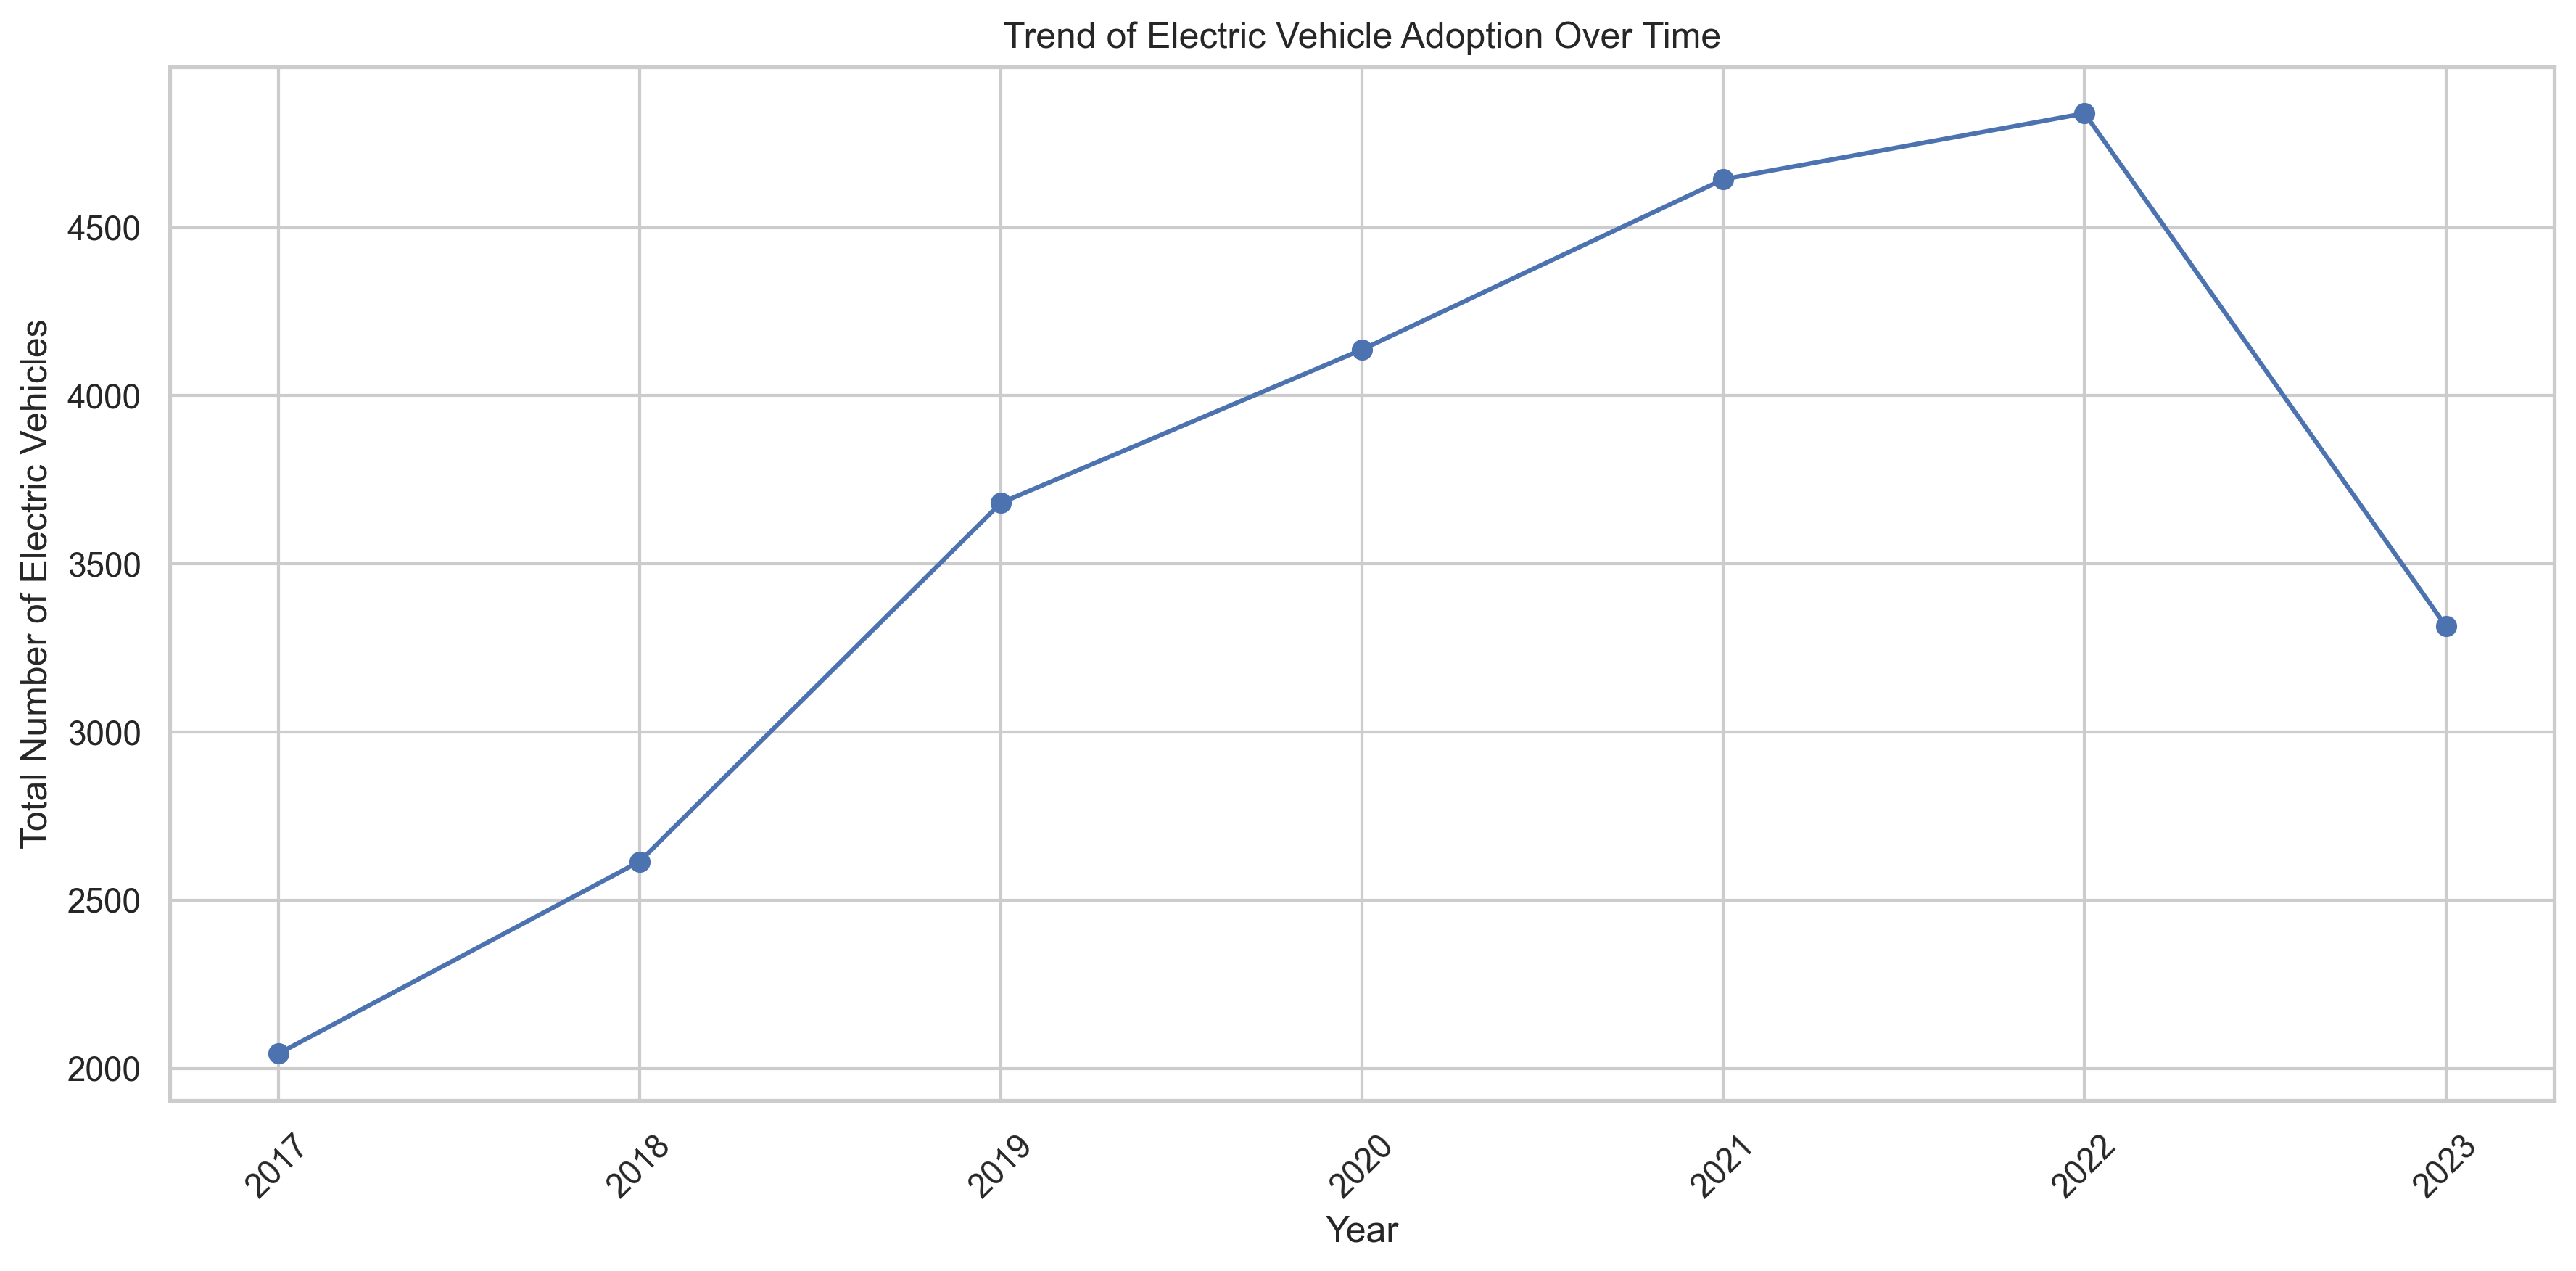
\includegraphics{SummaryPaper_FinalProject_T1_files/figure-pdf/cell-10-output-1.png}

}

\end{figure}

\begin{figure}[H]

{\centering 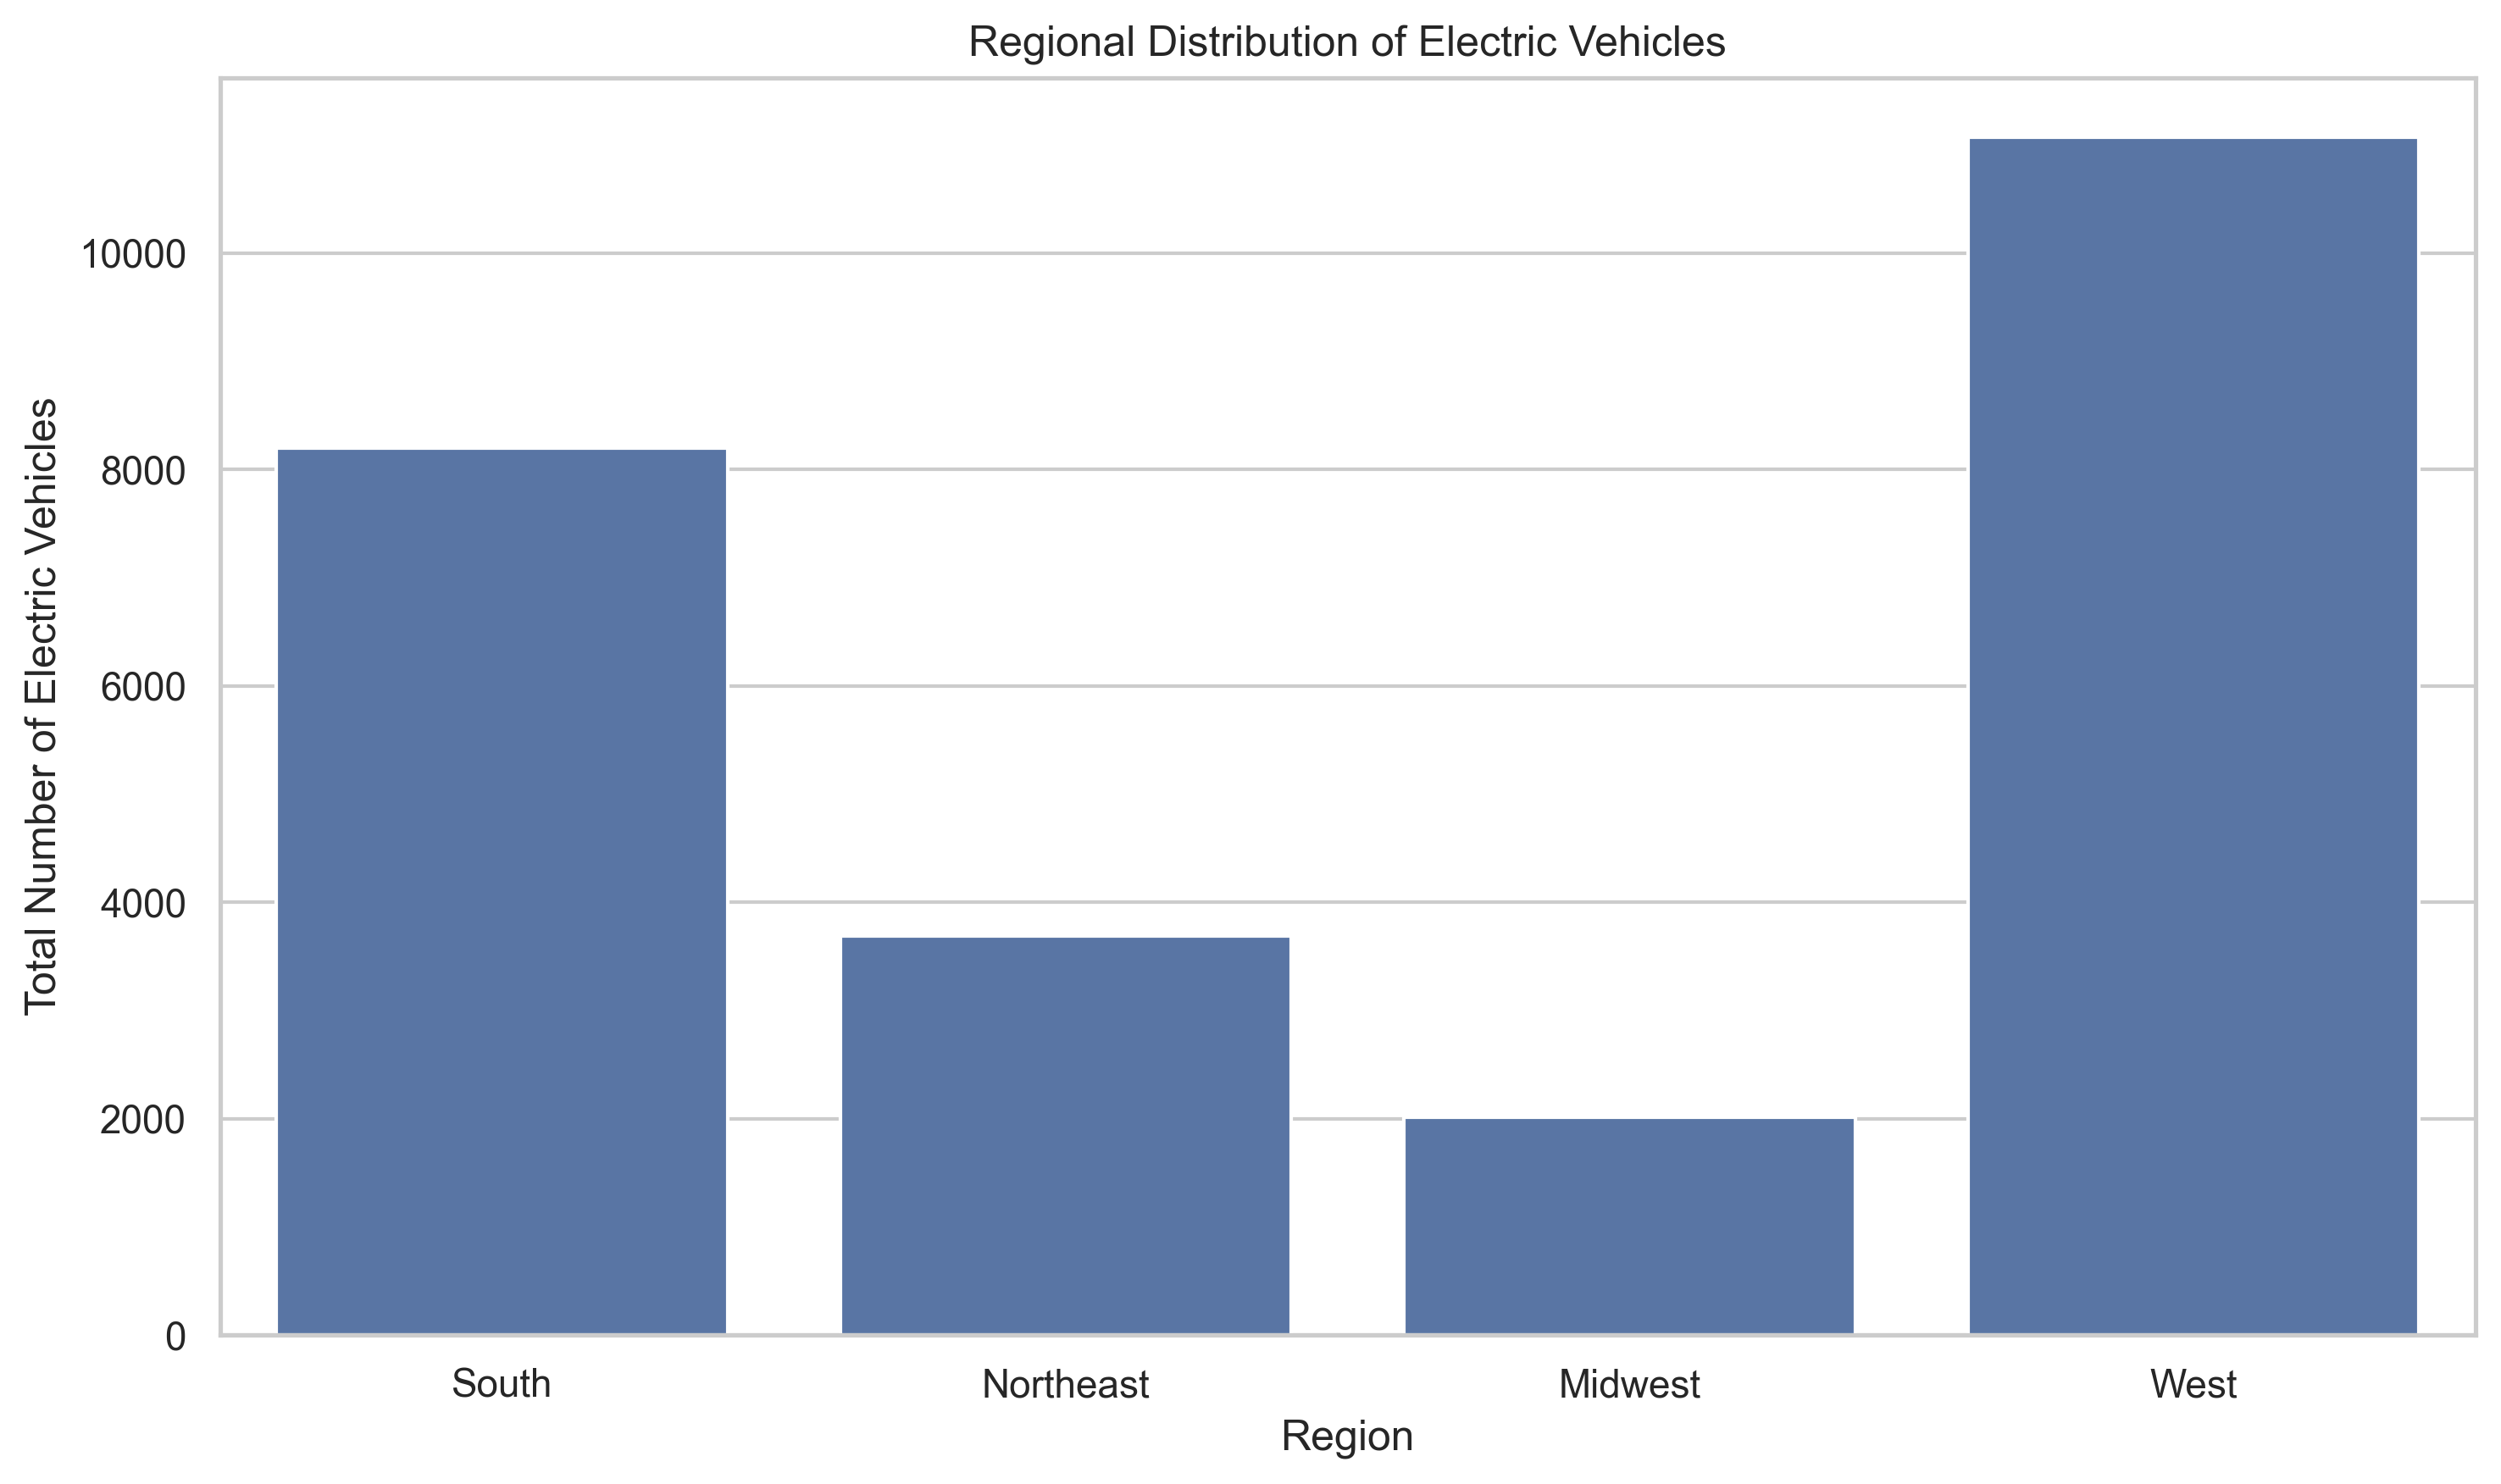
\includegraphics{SummaryPaper_FinalProject_T1_files/figure-pdf/cell-10-output-2.png}

}

\end{figure}

\textbf{Observation:} \textbf{Trend of Electric Vehicle Adoption Over
Time:} From 2017 to 2021, the line chart shows a consistent upward
trajectory in electric vehicle adoption, indicating robust growth. The
drop in 2023 suggests a possible market contraction or reporting anomaly
that should be investigated further.

\textbf{Regional Distribution of Electric Vehicles:} This bar chart
shows a significant regional variation in EV adoption, with the West far
ahead. It emphasises the uneven adoption of electric vehicles, pointing
to regional preferences or disparities in infrastructure and policy
support.

\hypertarget{smart-question-1how-is-the-ev-trend-across-years-in-different-regions}{%
\subsection{SMART Question 1:How is the EV trend across years in
different
regions?}\label{smart-question-1how-is-the-ev-trend-across-years-in-different-regions}}

\begin{Shaded}
\begin{Highlighting}[]
\ImportTok{import}\NormalTok{ warnings}
\NormalTok{warnings.filterwarnings(}\StringTok{"ignore"}\NormalTok{)}
\CommentTok{\# Visualization: Trend of Electric Vehicles Over the Years by Region}
\NormalTok{plt.figure(figsize}\OperatorTok{=}\NormalTok{(}\DecValTok{14}\NormalTok{, }\DecValTok{7}\NormalTok{))}
\NormalTok{sns.lineplot(data}\OperatorTok{=}\NormalTok{df, x}\OperatorTok{=}\StringTok{\textquotesingle{}Year\textquotesingle{}}\NormalTok{, y}\OperatorTok{=}\StringTok{\textquotesingle{}Electric Vehicle (EV) Total\textquotesingle{}}\NormalTok{, hue}\OperatorTok{=}\StringTok{\textquotesingle{}Region\textquotesingle{}}\NormalTok{, marker}\OperatorTok{=}\StringTok{\textquotesingle{}o\textquotesingle{}}\NormalTok{)}
\NormalTok{plt.title(}\StringTok{\textquotesingle{}Trend of Electric Vehicles Over the Years by Region\textquotesingle{}}\NormalTok{)}
\NormalTok{plt.xlabel(}\StringTok{\textquotesingle{}Year\textquotesingle{}}\NormalTok{)}
\NormalTok{plt.ylabel(}\StringTok{\textquotesingle{}Total Electric Vehicles\textquotesingle{}}\NormalTok{)}
\NormalTok{plt.legend(title}\OperatorTok{=}\StringTok{\textquotesingle{}Region\textquotesingle{}}\NormalTok{, loc}\OperatorTok{=}\StringTok{\textquotesingle{}upper left\textquotesingle{}}\NormalTok{)}
\NormalTok{plt.grid(}\VariableTok{True}\NormalTok{)}
\NormalTok{plt.show()}
\end{Highlighting}
\end{Shaded}

\begin{figure}[H]

{\centering 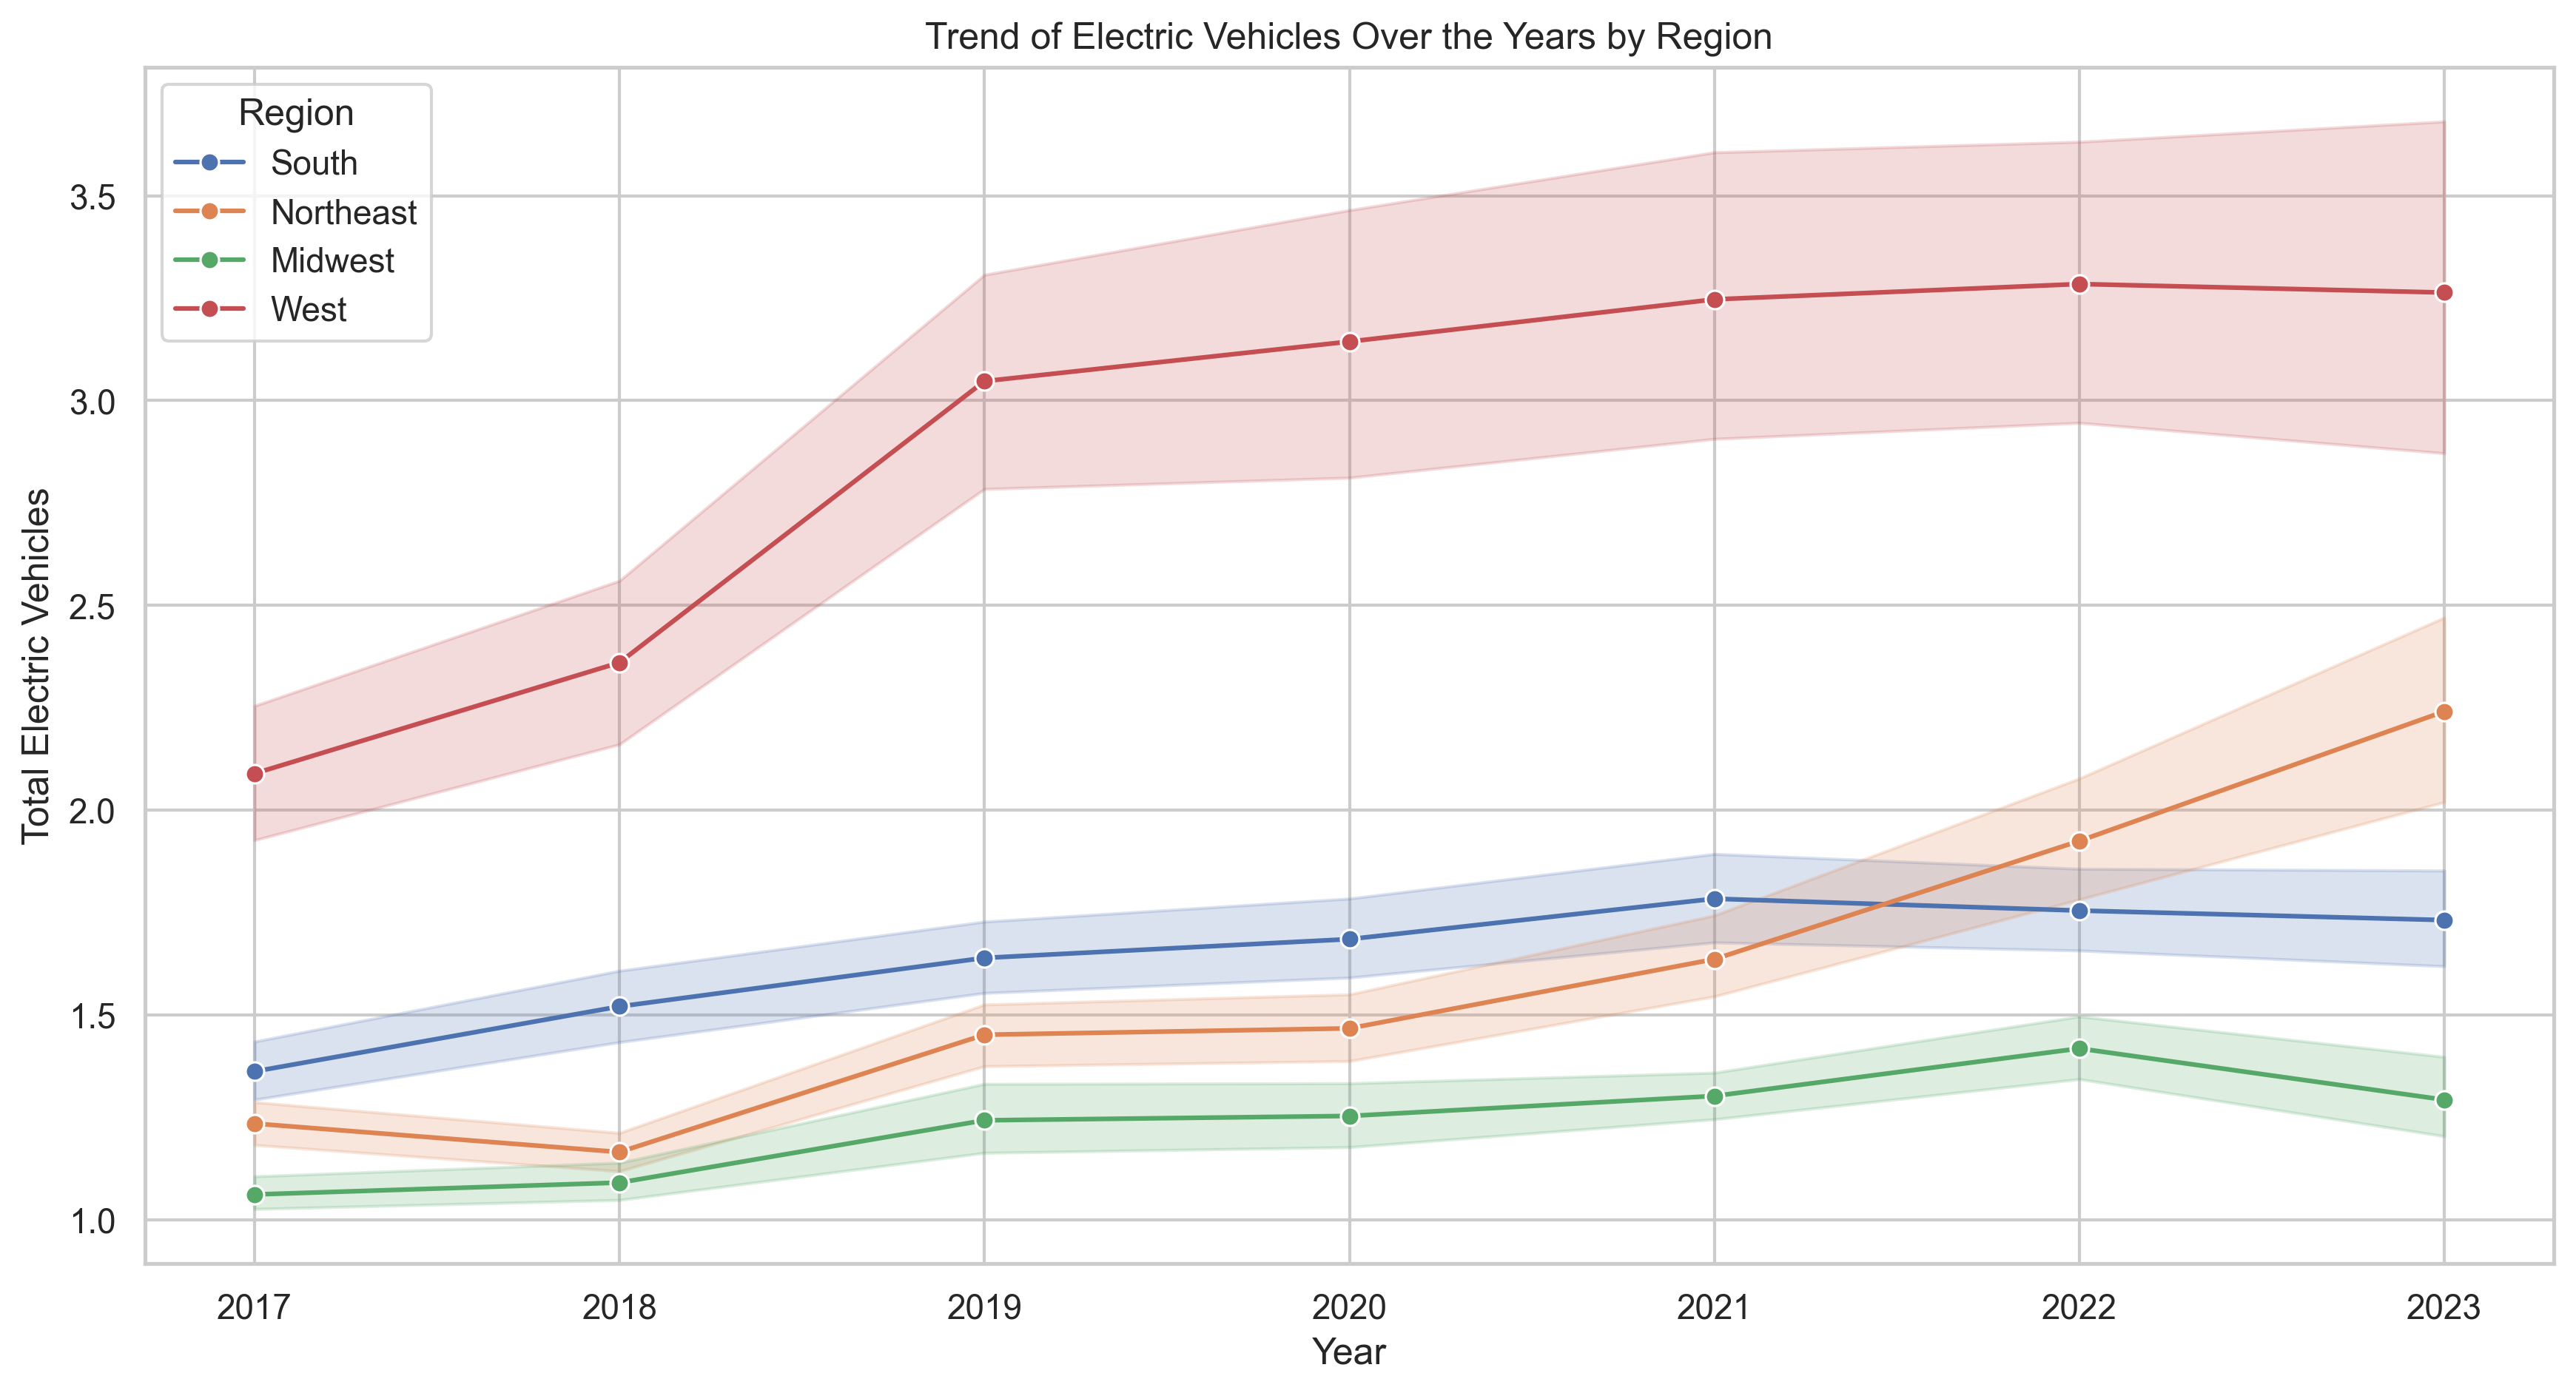
\includegraphics{SummaryPaper_FinalProject_T1_files/figure-pdf/cell-11-output-1.png}

}

\end{figure}

\textbf{Conclusion for the SMART Q1:} The multi-line chart with
confidence intervals demonstrates that, while all regions are
experiencing growth in EV adoption, the West region's pace is noticeably
faster. The graph also suggests that regional disparities in EV adoption
rates are increasing over time.

\hypertarget{checking-the-ev-adoption-in-the-top5-counties-from-each-region}{%
\subsection{Checking the EV adoption in the top5 counties from each
region}\label{checking-the-ev-adoption-in-the-top5-counties-from-each-region}}

\begin{Shaded}
\begin{Highlighting}[]
\ImportTok{import}\NormalTok{ warnings}
\NormalTok{warnings.filterwarnings(}\StringTok{"ignore"}\NormalTok{)}
\KeywordTok{def}\NormalTok{ plot\_top\_5\_counties\_for\_region(dataframe, region\_name):}
    \CommentTok{\# Filter for the current region}
\NormalTok{    region\_df }\OperatorTok{=}\NormalTok{ dataframe[dataframe[}\StringTok{\textquotesingle{}Region\textquotesingle{}}\NormalTok{] }\OperatorTok{==}\NormalTok{ region\_name]}

    \CommentTok{\# Group by \textquotesingle{}County\textquotesingle{} and sum up the EV totals}
\NormalTok{    ev\_totals }\OperatorTok{=}\NormalTok{ region\_df.groupby(}\StringTok{\textquotesingle{}County\textquotesingle{}}\NormalTok{)[}\StringTok{\textquotesingle{}Electric Vehicle (EV) Total\textquotesingle{}}\NormalTok{].}\BuiltInTok{sum}\NormalTok{()}

    \CommentTok{\# Sort and get the top 5 counties}
\NormalTok{    top\_5\_counties }\OperatorTok{=}\NormalTok{ ev\_totals.nlargest(}\DecValTok{5}\NormalTok{)}

    \CommentTok{\# Create the bar chart}
\NormalTok{    sns.barplot(x}\OperatorTok{=}\NormalTok{top\_5\_counties.index, y}\OperatorTok{=}\NormalTok{top\_5\_counties.values, palette}\OperatorTok{=}\StringTok{\textquotesingle{}viridis\textquotesingle{}}\NormalTok{)}
\NormalTok{    plt.title(}\SpecialStringTok{f\textquotesingle{}Top 5 Counties in EV Adoption in }\SpecialCharTok{\{}\NormalTok{region\_name}\SpecialCharTok{\}}\SpecialStringTok{ Region\textquotesingle{}}\NormalTok{)}
\NormalTok{    plt.xlabel(}\StringTok{\textquotesingle{}County\textquotesingle{}}\NormalTok{)}
\NormalTok{    plt.ylabel(}\StringTok{\textquotesingle{}Total EVs\textquotesingle{}}\NormalTok{)}
\NormalTok{    plt.xticks(rotation}\OperatorTok{=}\DecValTok{45}\NormalTok{)}

\CommentTok{\# Plot for a single region as an example}
\NormalTok{plt.figure(figsize}\OperatorTok{=}\NormalTok{(}\DecValTok{12}\NormalTok{, }\DecValTok{6}\NormalTok{))}
\NormalTok{plot\_top\_5\_counties\_for\_region(df, }\StringTok{\textquotesingle{}South\textquotesingle{}}\NormalTok{)}
\NormalTok{plt.show()}
\end{Highlighting}
\end{Shaded}

\begin{figure}[H]

{\centering 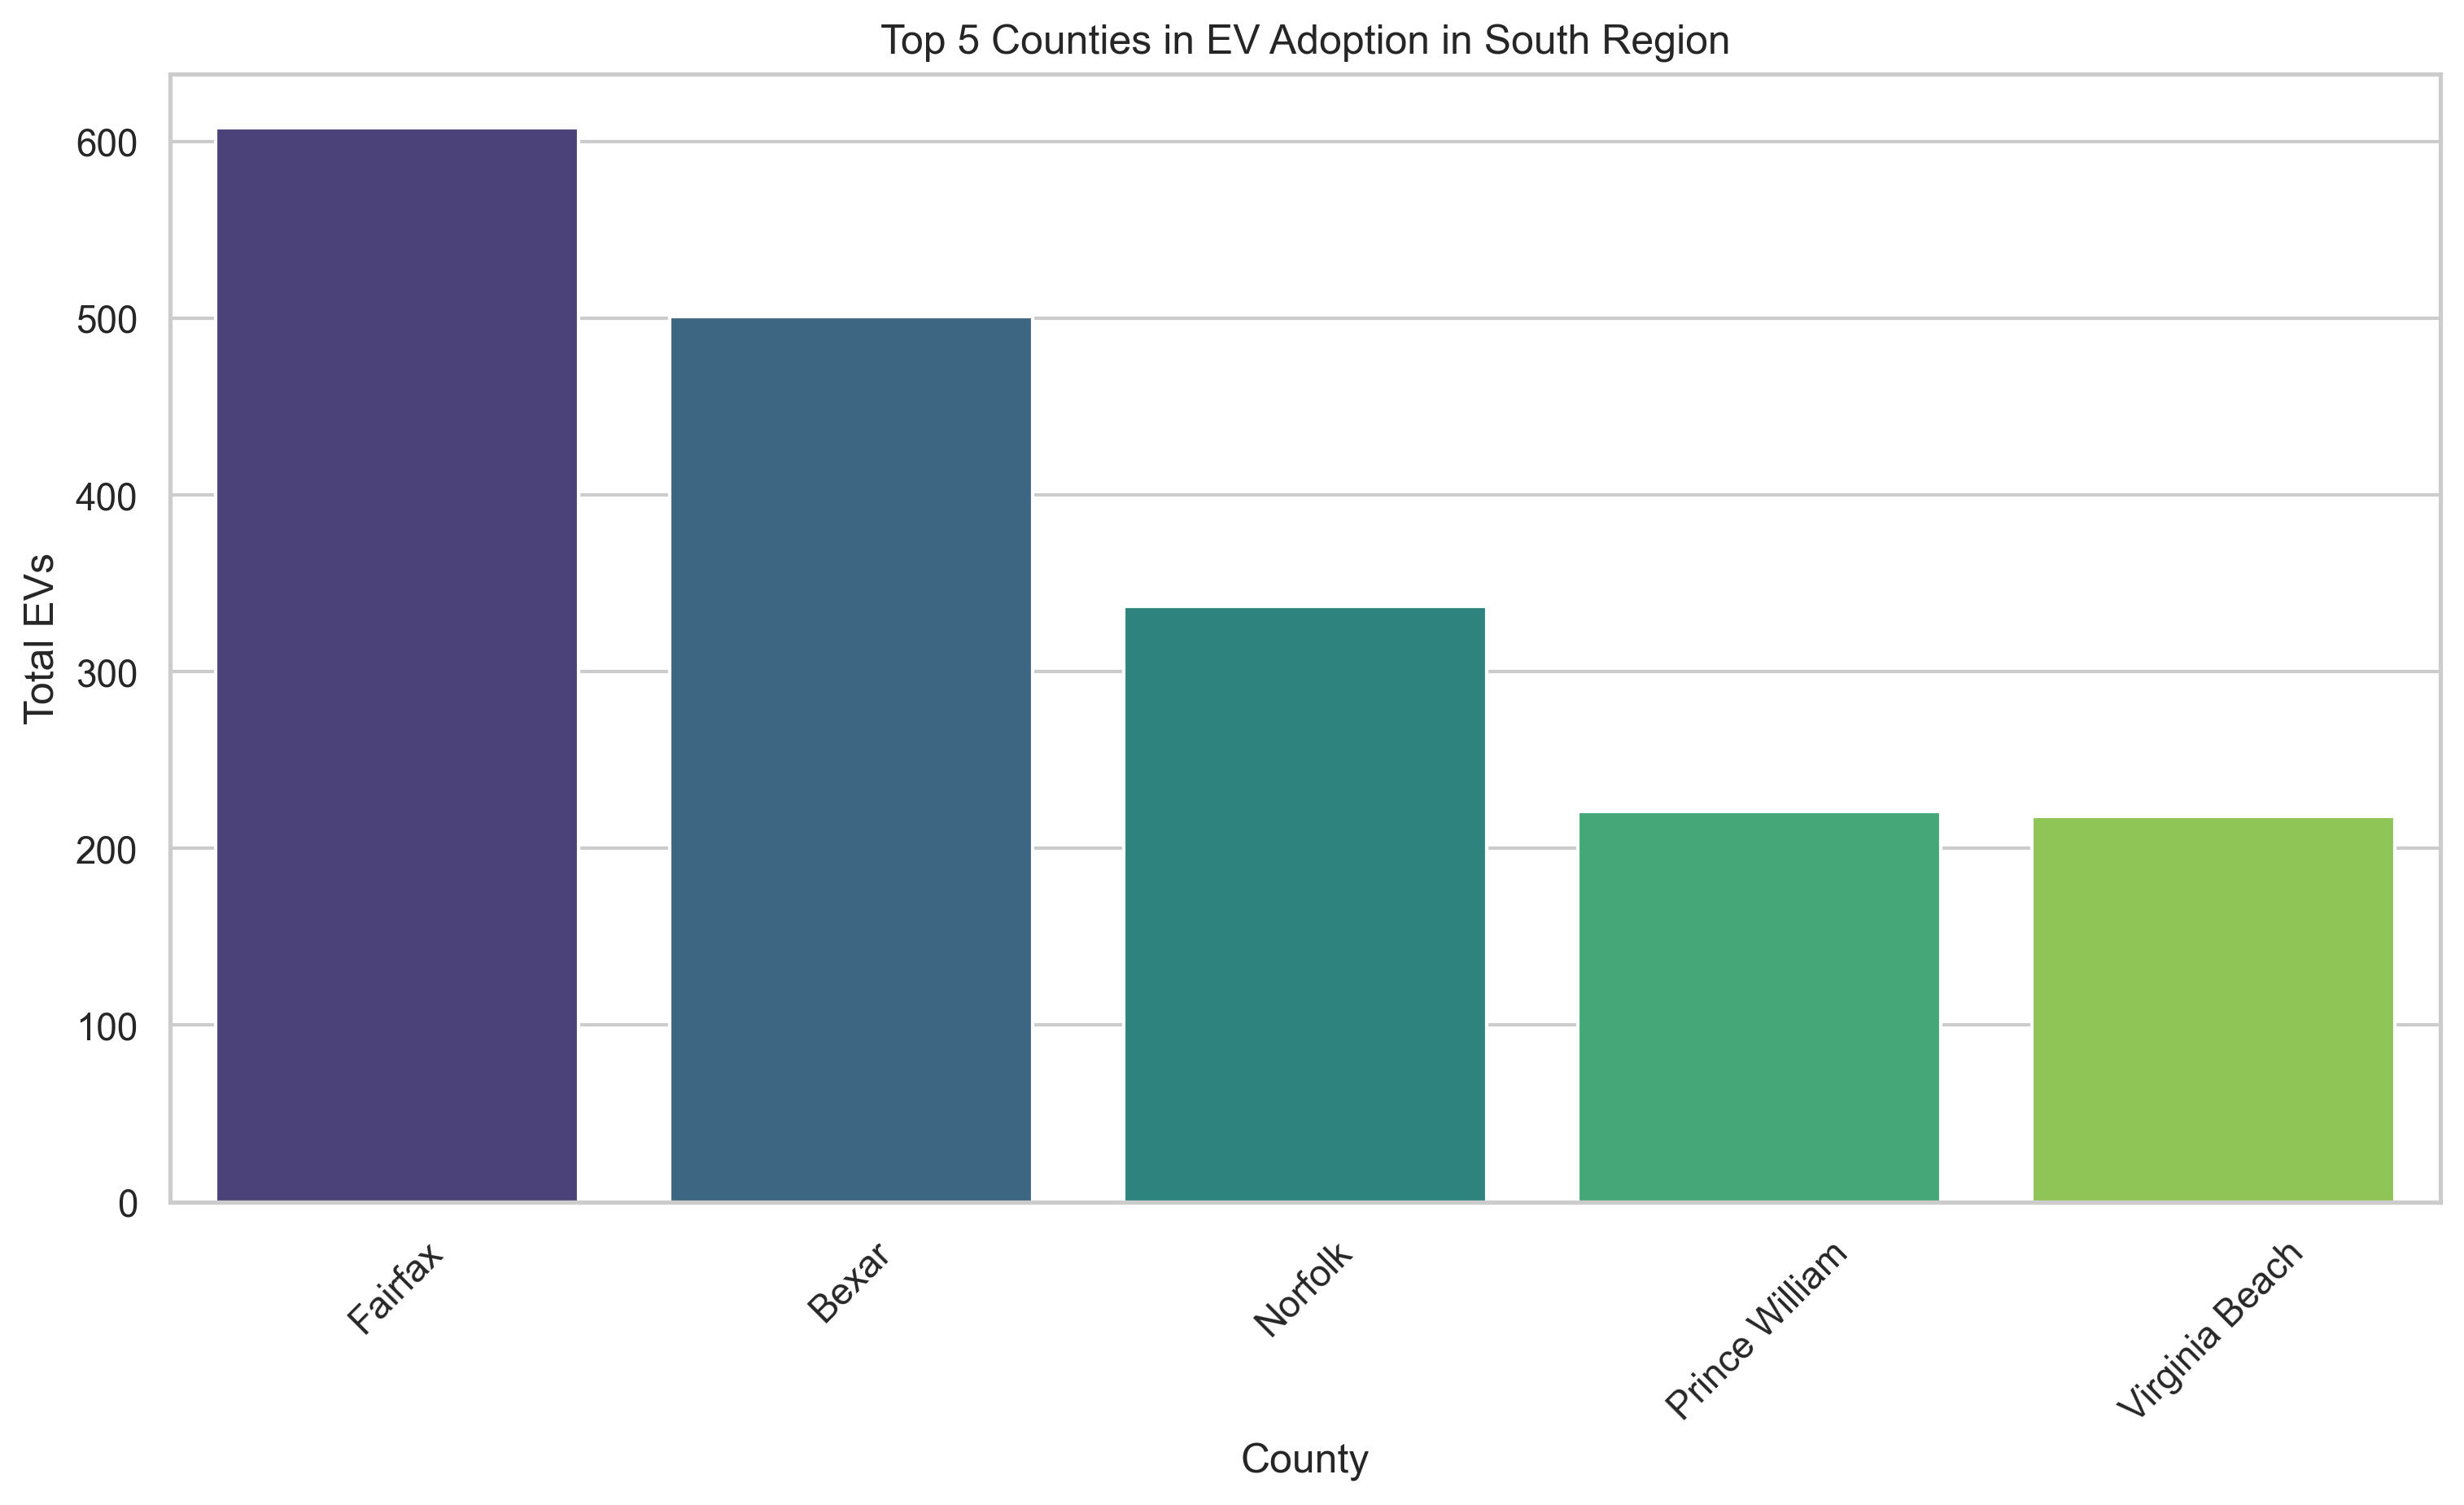
\includegraphics{SummaryPaper_FinalProject_T1_files/figure-pdf/cell-12-output-1.png}

}

\end{figure}

\textbf{Observation:} The bar chart indicates Fairfax County leads in EV
adoption within the South region, followed by Bexar and others. This may
reflect differing economic dynamics, policy incentives, or consumer
behaviors at the county level within the region.

\begin{Shaded}
\begin{Highlighting}[]
\ImportTok{import}\NormalTok{ warnings}
\NormalTok{warnings.filterwarnings(}\StringTok{"ignore"}\NormalTok{)}
\NormalTok{plt.figure(figsize}\OperatorTok{=}\NormalTok{(}\DecValTok{12}\NormalTok{, }\DecValTok{6}\NormalTok{))}
\NormalTok{plot\_top\_5\_counties\_for\_region(df, }\StringTok{\textquotesingle{}Midwest\textquotesingle{}}\NormalTok{)}
\NormalTok{plt.show()}
\end{Highlighting}
\end{Shaded}

\begin{figure}[H]

{\centering 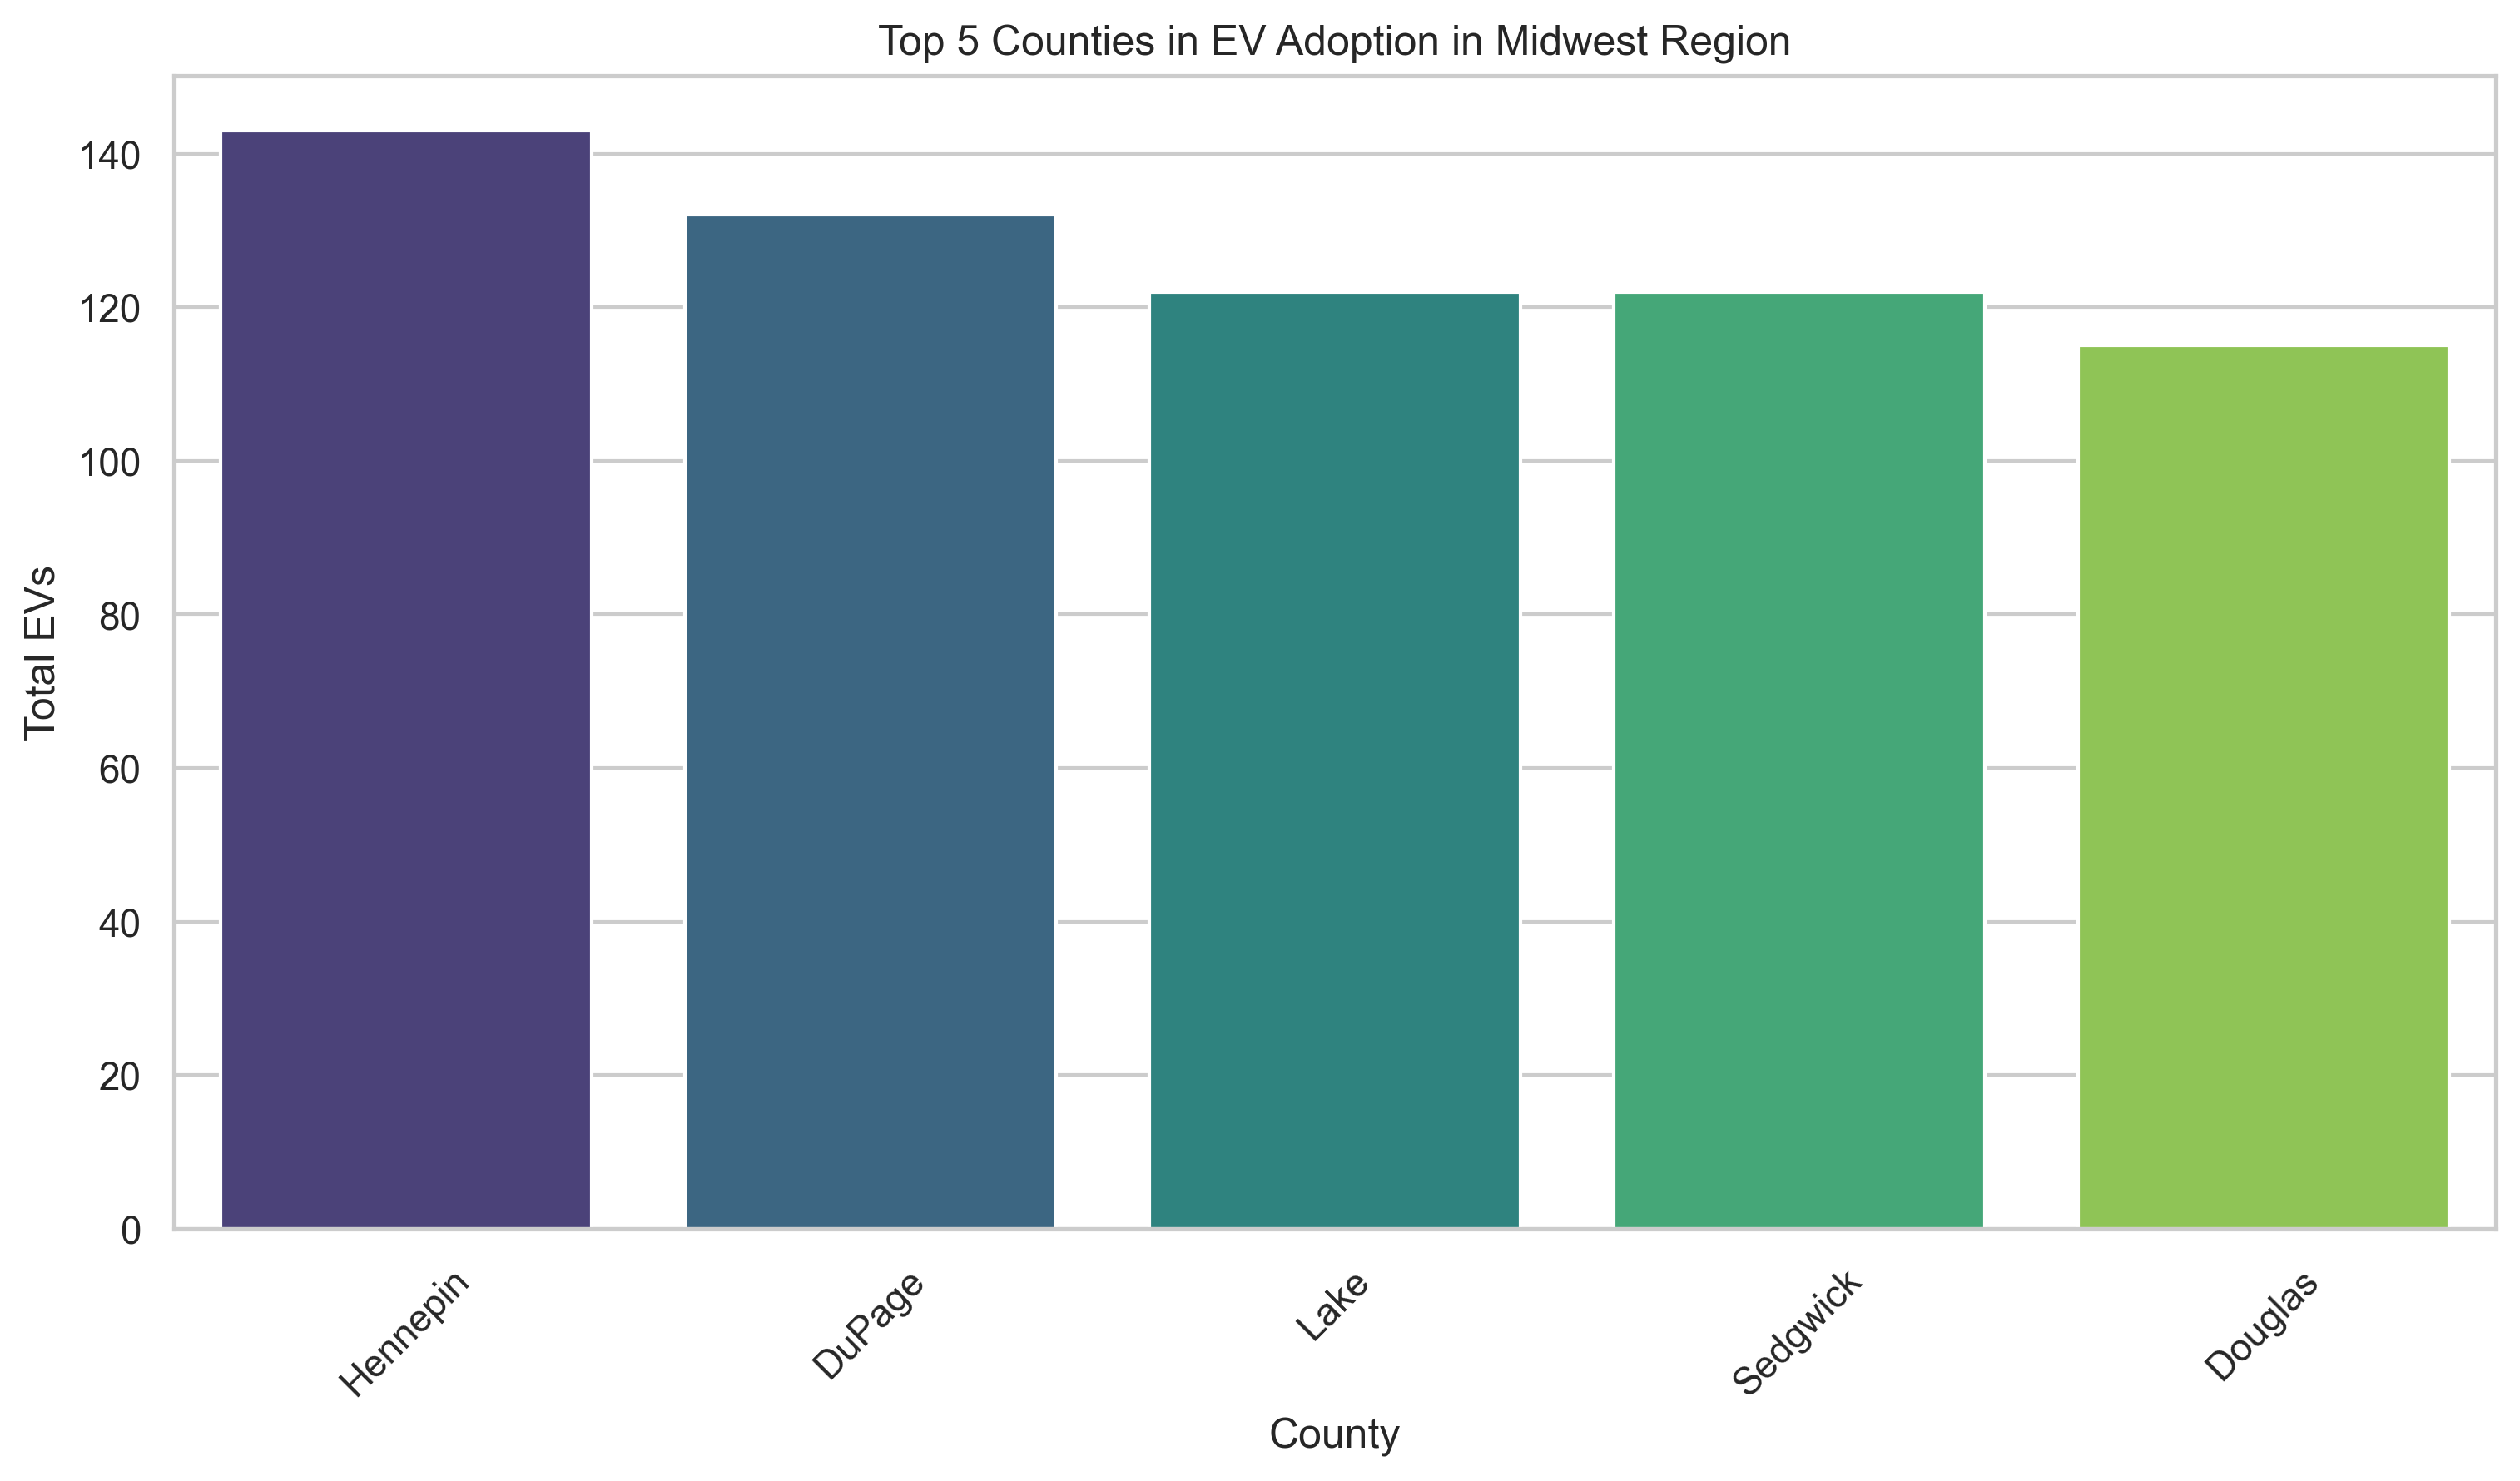
\includegraphics{SummaryPaper_FinalProject_T1_files/figure-pdf/cell-13-output-1.png}

}

\end{figure}

\textbf{Observation:} The top counties in the Midwest region have a more
even distribution of EV adoption. Hennepin and Page counties lead, with
Douglas close behind, indicating a more homogeneous adoption pattern
among the top performers in this region.

\begin{Shaded}
\begin{Highlighting}[]
\ImportTok{import}\NormalTok{ warnings}
\NormalTok{warnings.filterwarnings(}\StringTok{"ignore"}\NormalTok{)}
\NormalTok{plt.figure(figsize}\OperatorTok{=}\NormalTok{(}\DecValTok{12}\NormalTok{, }\DecValTok{6}\NormalTok{))}
\NormalTok{plot\_top\_5\_counties\_for\_region(df, }\StringTok{\textquotesingle{}West\textquotesingle{}}\NormalTok{)}
\NormalTok{plt.show()}
\end{Highlighting}
\end{Shaded}

\begin{figure}[H]

{\centering 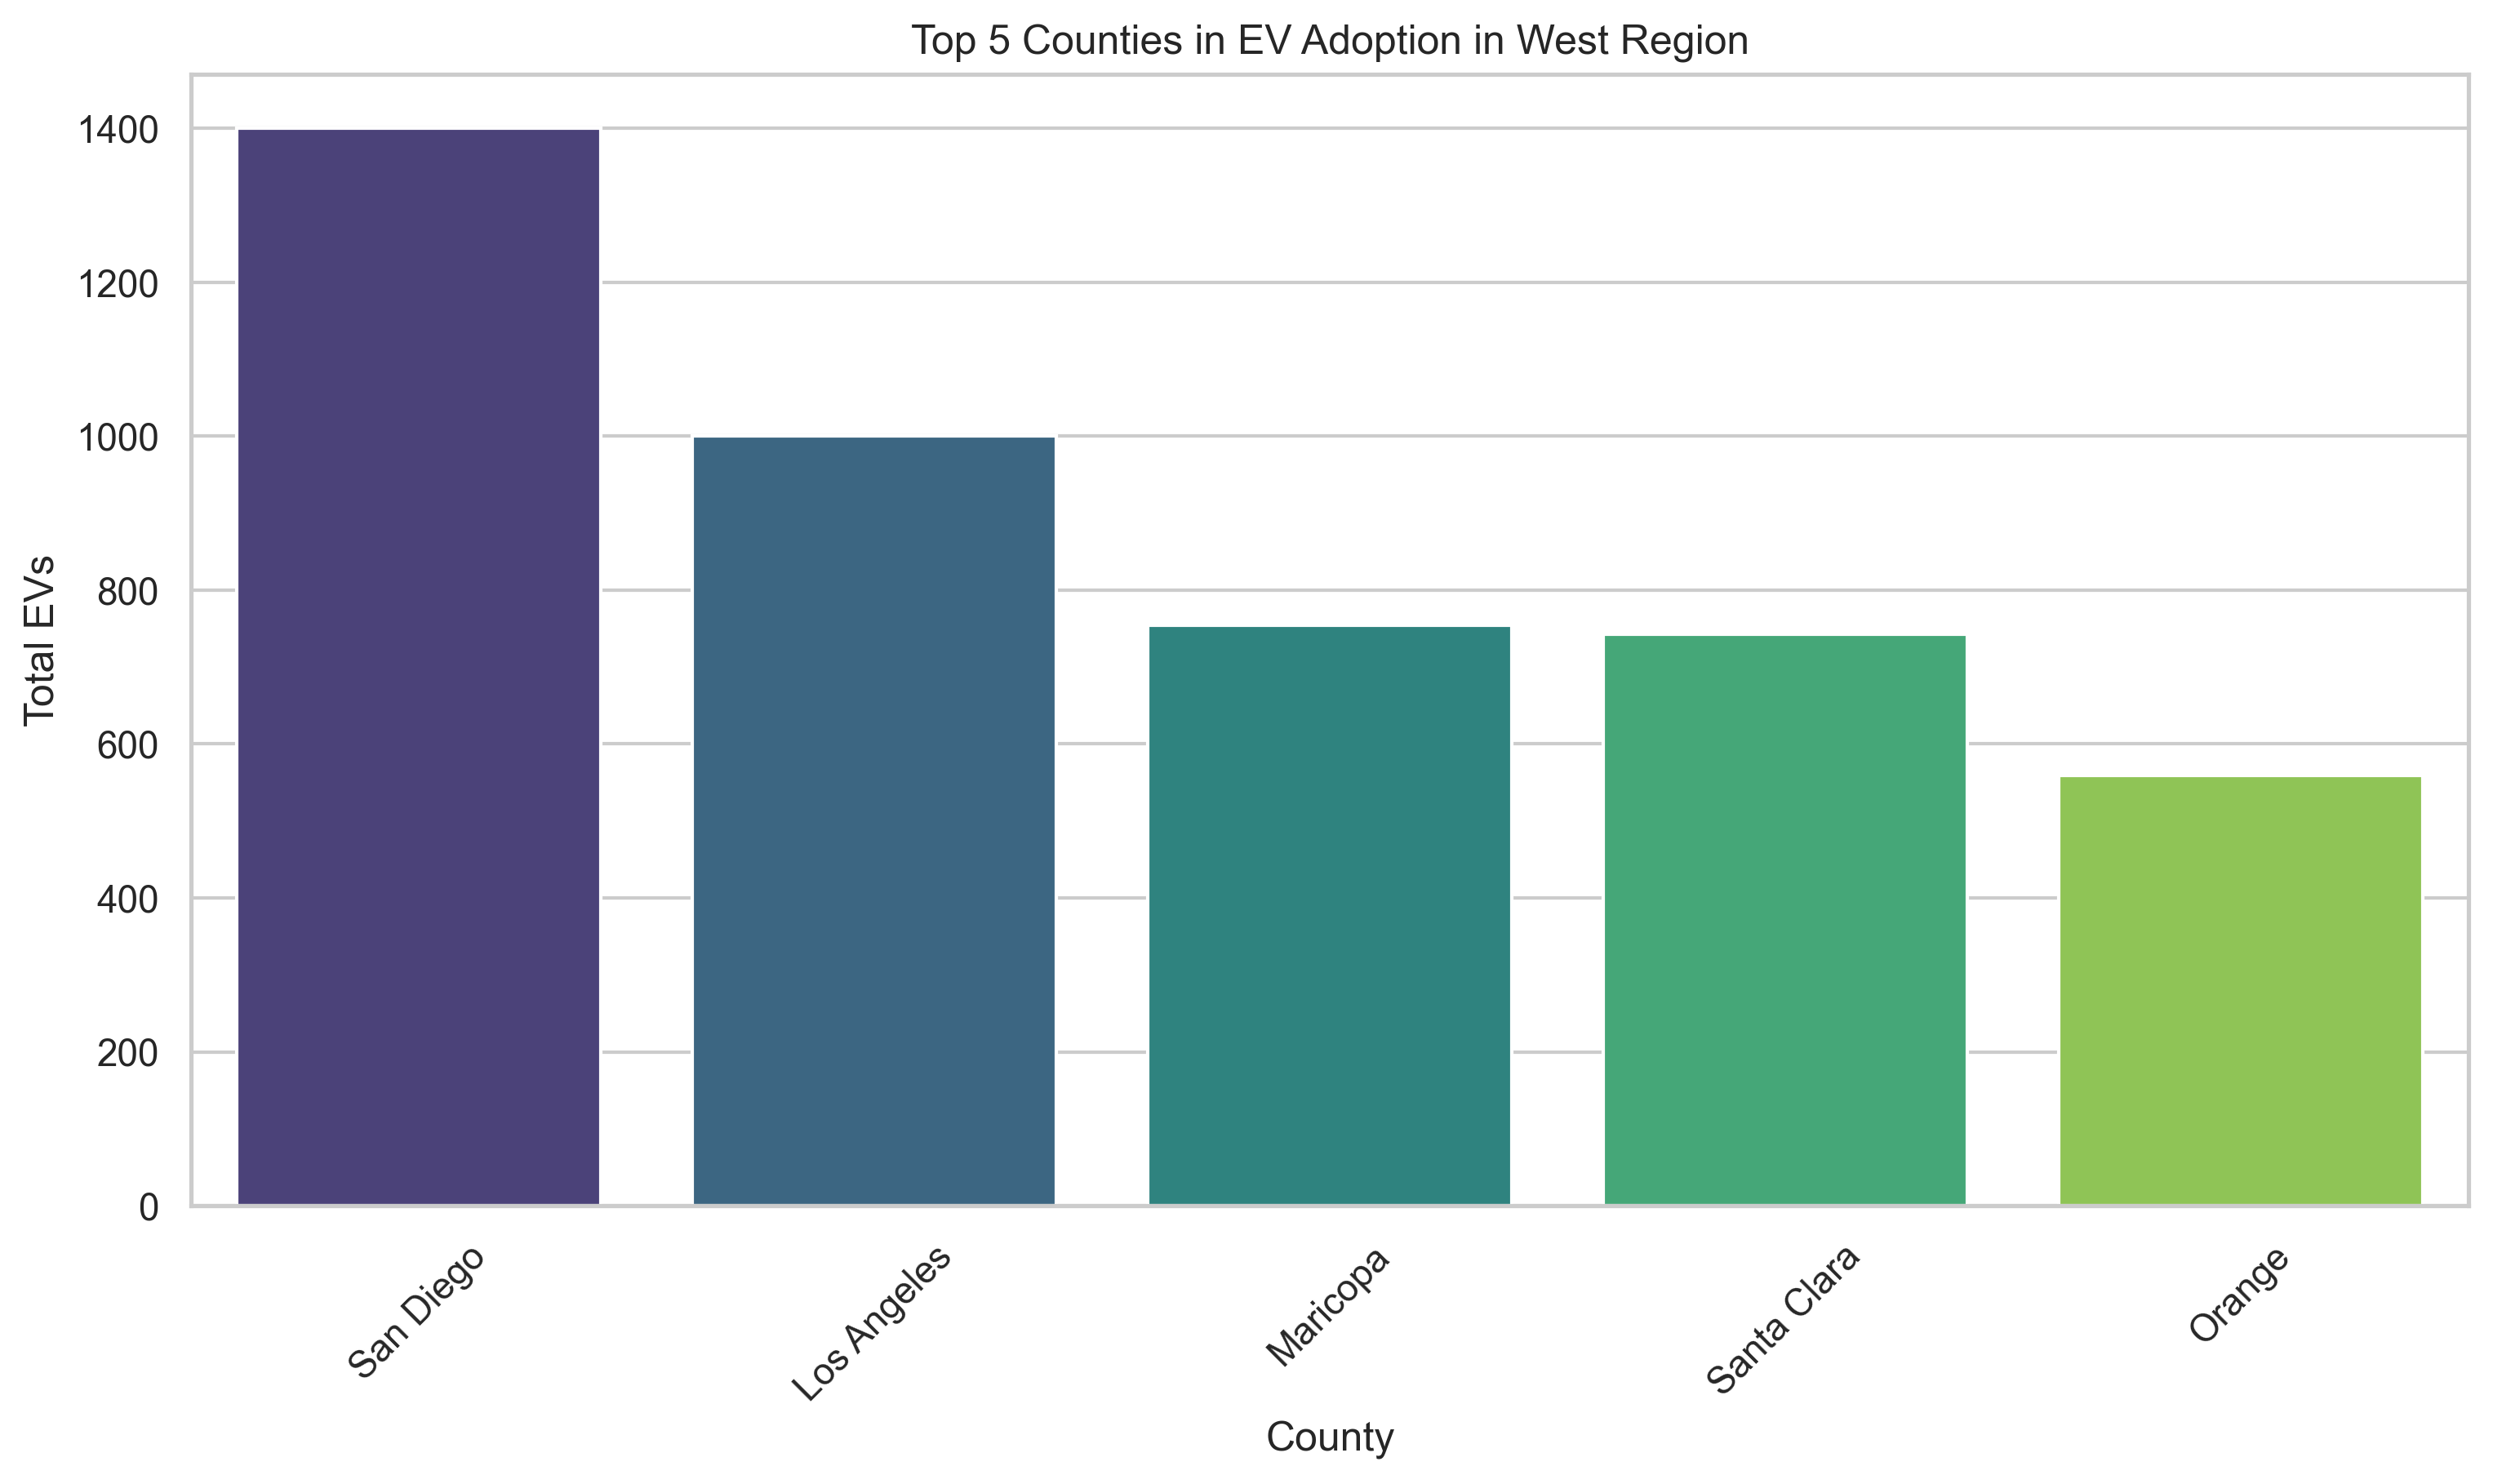
\includegraphics{SummaryPaper_FinalProject_T1_files/figure-pdf/cell-14-output-1.png}

}

\end{figure}

\textbf{Observation:} San Diego leads the West in EV adoption, with
significant contributions from Los Angeles and Santa Clara. The chart
indicates that California's urban counties have a high concentration of
EVs, most likely due to favourable policies and infrastructure.

\hypertarget{eda-of-bev-and-phevs}{%
\section{EDA of BEV AND PHEV's}\label{eda-of-bev-and-phevs}}

\begin{Shaded}
\begin{Highlighting}[]
\ImportTok{import}\NormalTok{ warnings}
\NormalTok{warnings.filterwarnings(}\StringTok{"ignore"}\NormalTok{)}
\CommentTok{\# Grouping the data by state and summing up the BEVs and PHEVs}
\NormalTok{state\_ev\_totals }\OperatorTok{=}\NormalTok{ df.groupby(}\StringTok{\textquotesingle{}State\textquotesingle{}}\NormalTok{)[[}\StringTok{\textquotesingle{}Battery Electric Vehicles (BEVs)\textquotesingle{}}\NormalTok{, }\StringTok{\textquotesingle{}Plug{-}In Hybrid Electric Vehicles (PHEVs)\textquotesingle{}}\NormalTok{]].}\BuiltInTok{sum}\NormalTok{()}

\CommentTok{\# Sorting the states based on the total number of EVs (BEVs + PHEVs)}
\NormalTok{state\_ev\_totals[}\StringTok{\textquotesingle{}Total EVs\textquotesingle{}}\NormalTok{] }\OperatorTok{=}\NormalTok{ state\_ev\_totals[}\StringTok{\textquotesingle{}Battery Electric Vehicles (BEVs)\textquotesingle{}}\NormalTok{] }\OperatorTok{+}\NormalTok{ state\_ev\_totals[}\StringTok{\textquotesingle{}Plug{-}In Hybrid Electric Vehicles (PHEVs)\textquotesingle{}}\NormalTok{]}
\NormalTok{state\_ev\_totals\_sorted }\OperatorTok{=}\NormalTok{ state\_ev\_totals.sort\_values(by}\OperatorTok{=}\StringTok{\textquotesingle{}Total EVs\textquotesingle{}}\NormalTok{, ascending}\OperatorTok{=}\VariableTok{False}\NormalTok{)}

\CommentTok{\# Plotting a stacked bar chart}
\NormalTok{state\_ev\_totals\_sorted[[}\StringTok{\textquotesingle{}Battery Electric Vehicles (BEVs)\textquotesingle{}}\NormalTok{, }\StringTok{\textquotesingle{}Plug{-}In Hybrid Electric Vehicles (PHEVs)\textquotesingle{}}\NormalTok{]].plot(kind}\OperatorTok{=}\StringTok{\textquotesingle{}bar\textquotesingle{}}\NormalTok{, stacked}\OperatorTok{=}\VariableTok{True}\NormalTok{, figsize}\OperatorTok{=}\NormalTok{(}\DecValTok{15}\NormalTok{, }\DecValTok{8}\NormalTok{))}
\NormalTok{plt.title(}\StringTok{\textquotesingle{}Adoption of BEVs and PHEVs by State\textquotesingle{}}\NormalTok{)}
\NormalTok{plt.xlabel(}\StringTok{\textquotesingle{}State\textquotesingle{}}\NormalTok{)}
\NormalTok{plt.ylabel(}\StringTok{\textquotesingle{}Number of Electric Vehicles\textquotesingle{}}\NormalTok{)}
\NormalTok{plt.legend(title}\OperatorTok{=}\StringTok{\textquotesingle{}Vehicle Type\textquotesingle{}}\NormalTok{)}
\NormalTok{plt.tight\_layout()}

\CommentTok{\# Display the plot}
\NormalTok{plt.show()}
\end{Highlighting}
\end{Shaded}

\begin{figure}[H]

{\centering 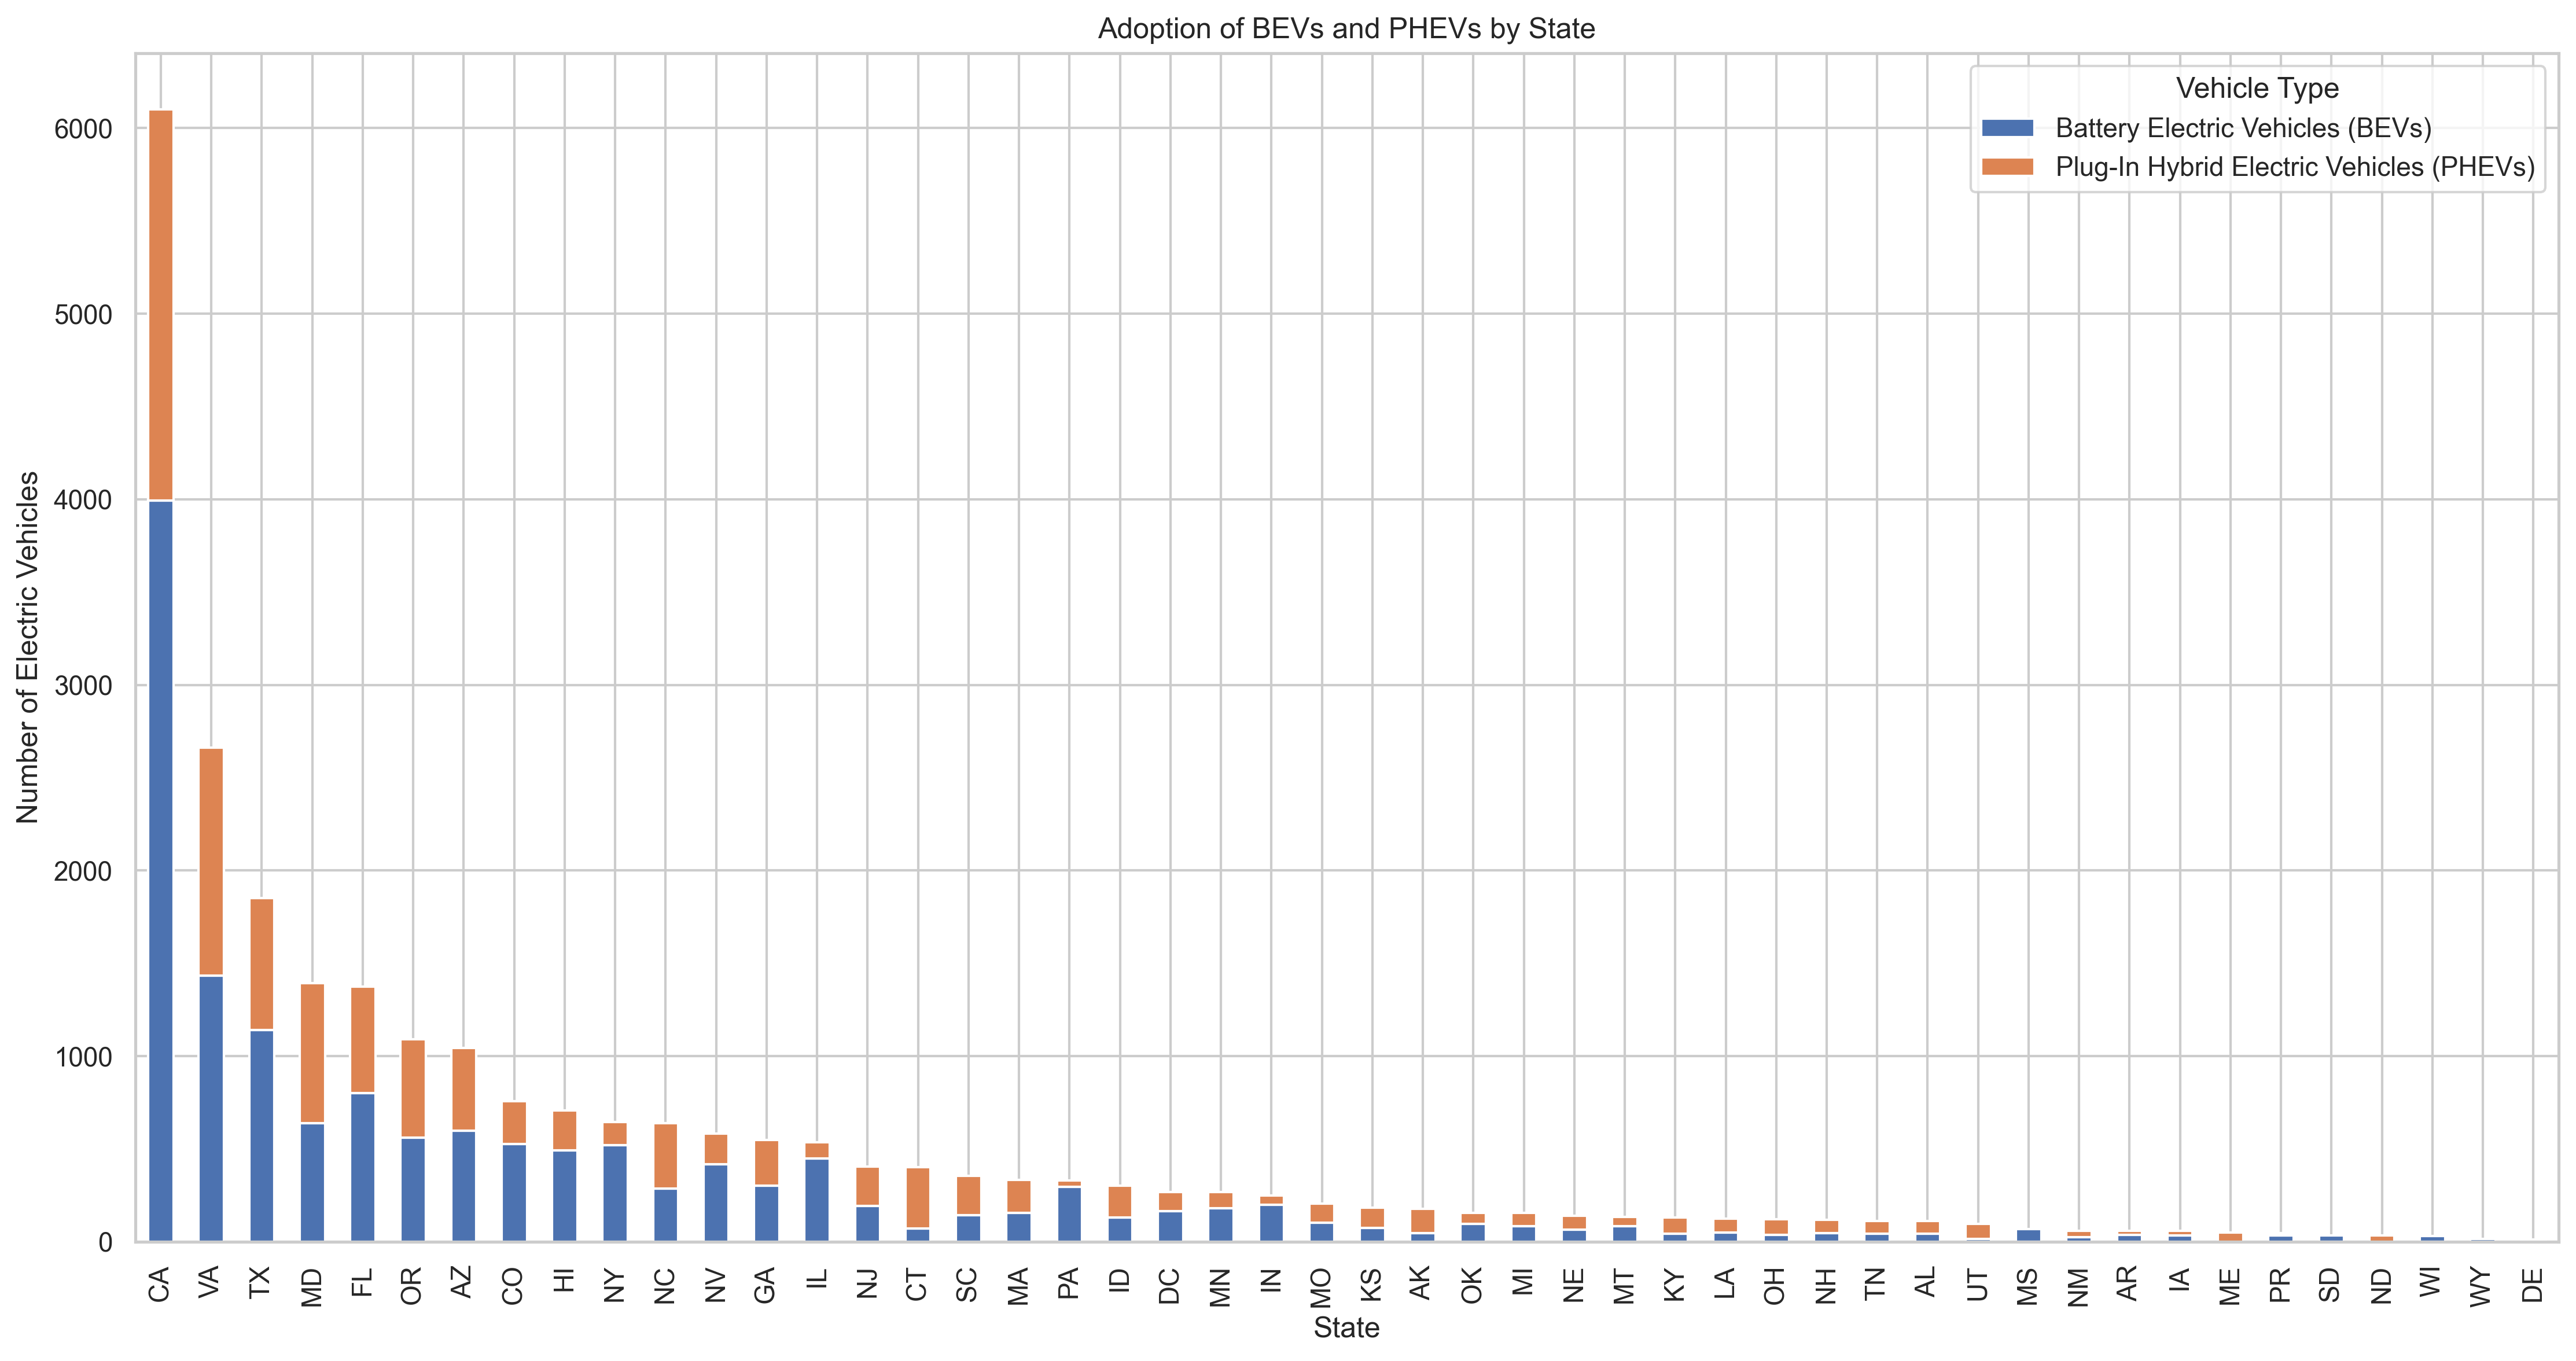
\includegraphics{SummaryPaper_FinalProject_T1_files/figure-pdf/cell-15-output-1.png}

}

\end{figure}

\textbf{Observation:} When compared to other states, California has a
significant lead in the adoption of both BEVs and PHEVs, reflecting its
pioneering role in EV adoption. This stacked bar chart highlights the
state's dominance in the EV market.

\begin{Shaded}
\begin{Highlighting}[]
\ImportTok{import}\NormalTok{ warnings}
\NormalTok{warnings.filterwarnings(}\StringTok{"ignore"}\NormalTok{)}
\CommentTok{\# Bar Chart of Average EVs by State}
\NormalTok{average\_evs\_by\_state }\OperatorTok{=}\NormalTok{ df.groupby(}\StringTok{\textquotesingle{}State\textquotesingle{}}\NormalTok{)[}\StringTok{\textquotesingle{}Electric Vehicle (EV) Total\textquotesingle{}}\NormalTok{].mean().sort\_values(ascending}\OperatorTok{=}\VariableTok{False}\NormalTok{)}

\NormalTok{plt.figure(figsize}\OperatorTok{=}\NormalTok{(}\DecValTok{15}\NormalTok{, }\DecValTok{8}\NormalTok{))}
\NormalTok{average\_evs\_by\_state.plot(kind}\OperatorTok{=}\StringTok{\textquotesingle{}bar\textquotesingle{}}\NormalTok{, color}\OperatorTok{=}\StringTok{\textquotesingle{}skyblue\textquotesingle{}}\NormalTok{)}
\NormalTok{plt.title(}\StringTok{\textquotesingle{}Average Number of EVs by State\textquotesingle{}}\NormalTok{)}
\NormalTok{plt.xlabel(}\StringTok{\textquotesingle{}State\textquotesingle{}}\NormalTok{)}
\NormalTok{plt.ylabel(}\StringTok{\textquotesingle{}Average Number of EVs\textquotesingle{}}\NormalTok{)}
\NormalTok{plt.xticks(rotation}\OperatorTok{=}\DecValTok{45}\NormalTok{)}
\NormalTok{plt.show()}
\end{Highlighting}
\end{Shaded}

\begin{figure}[H]

{\centering 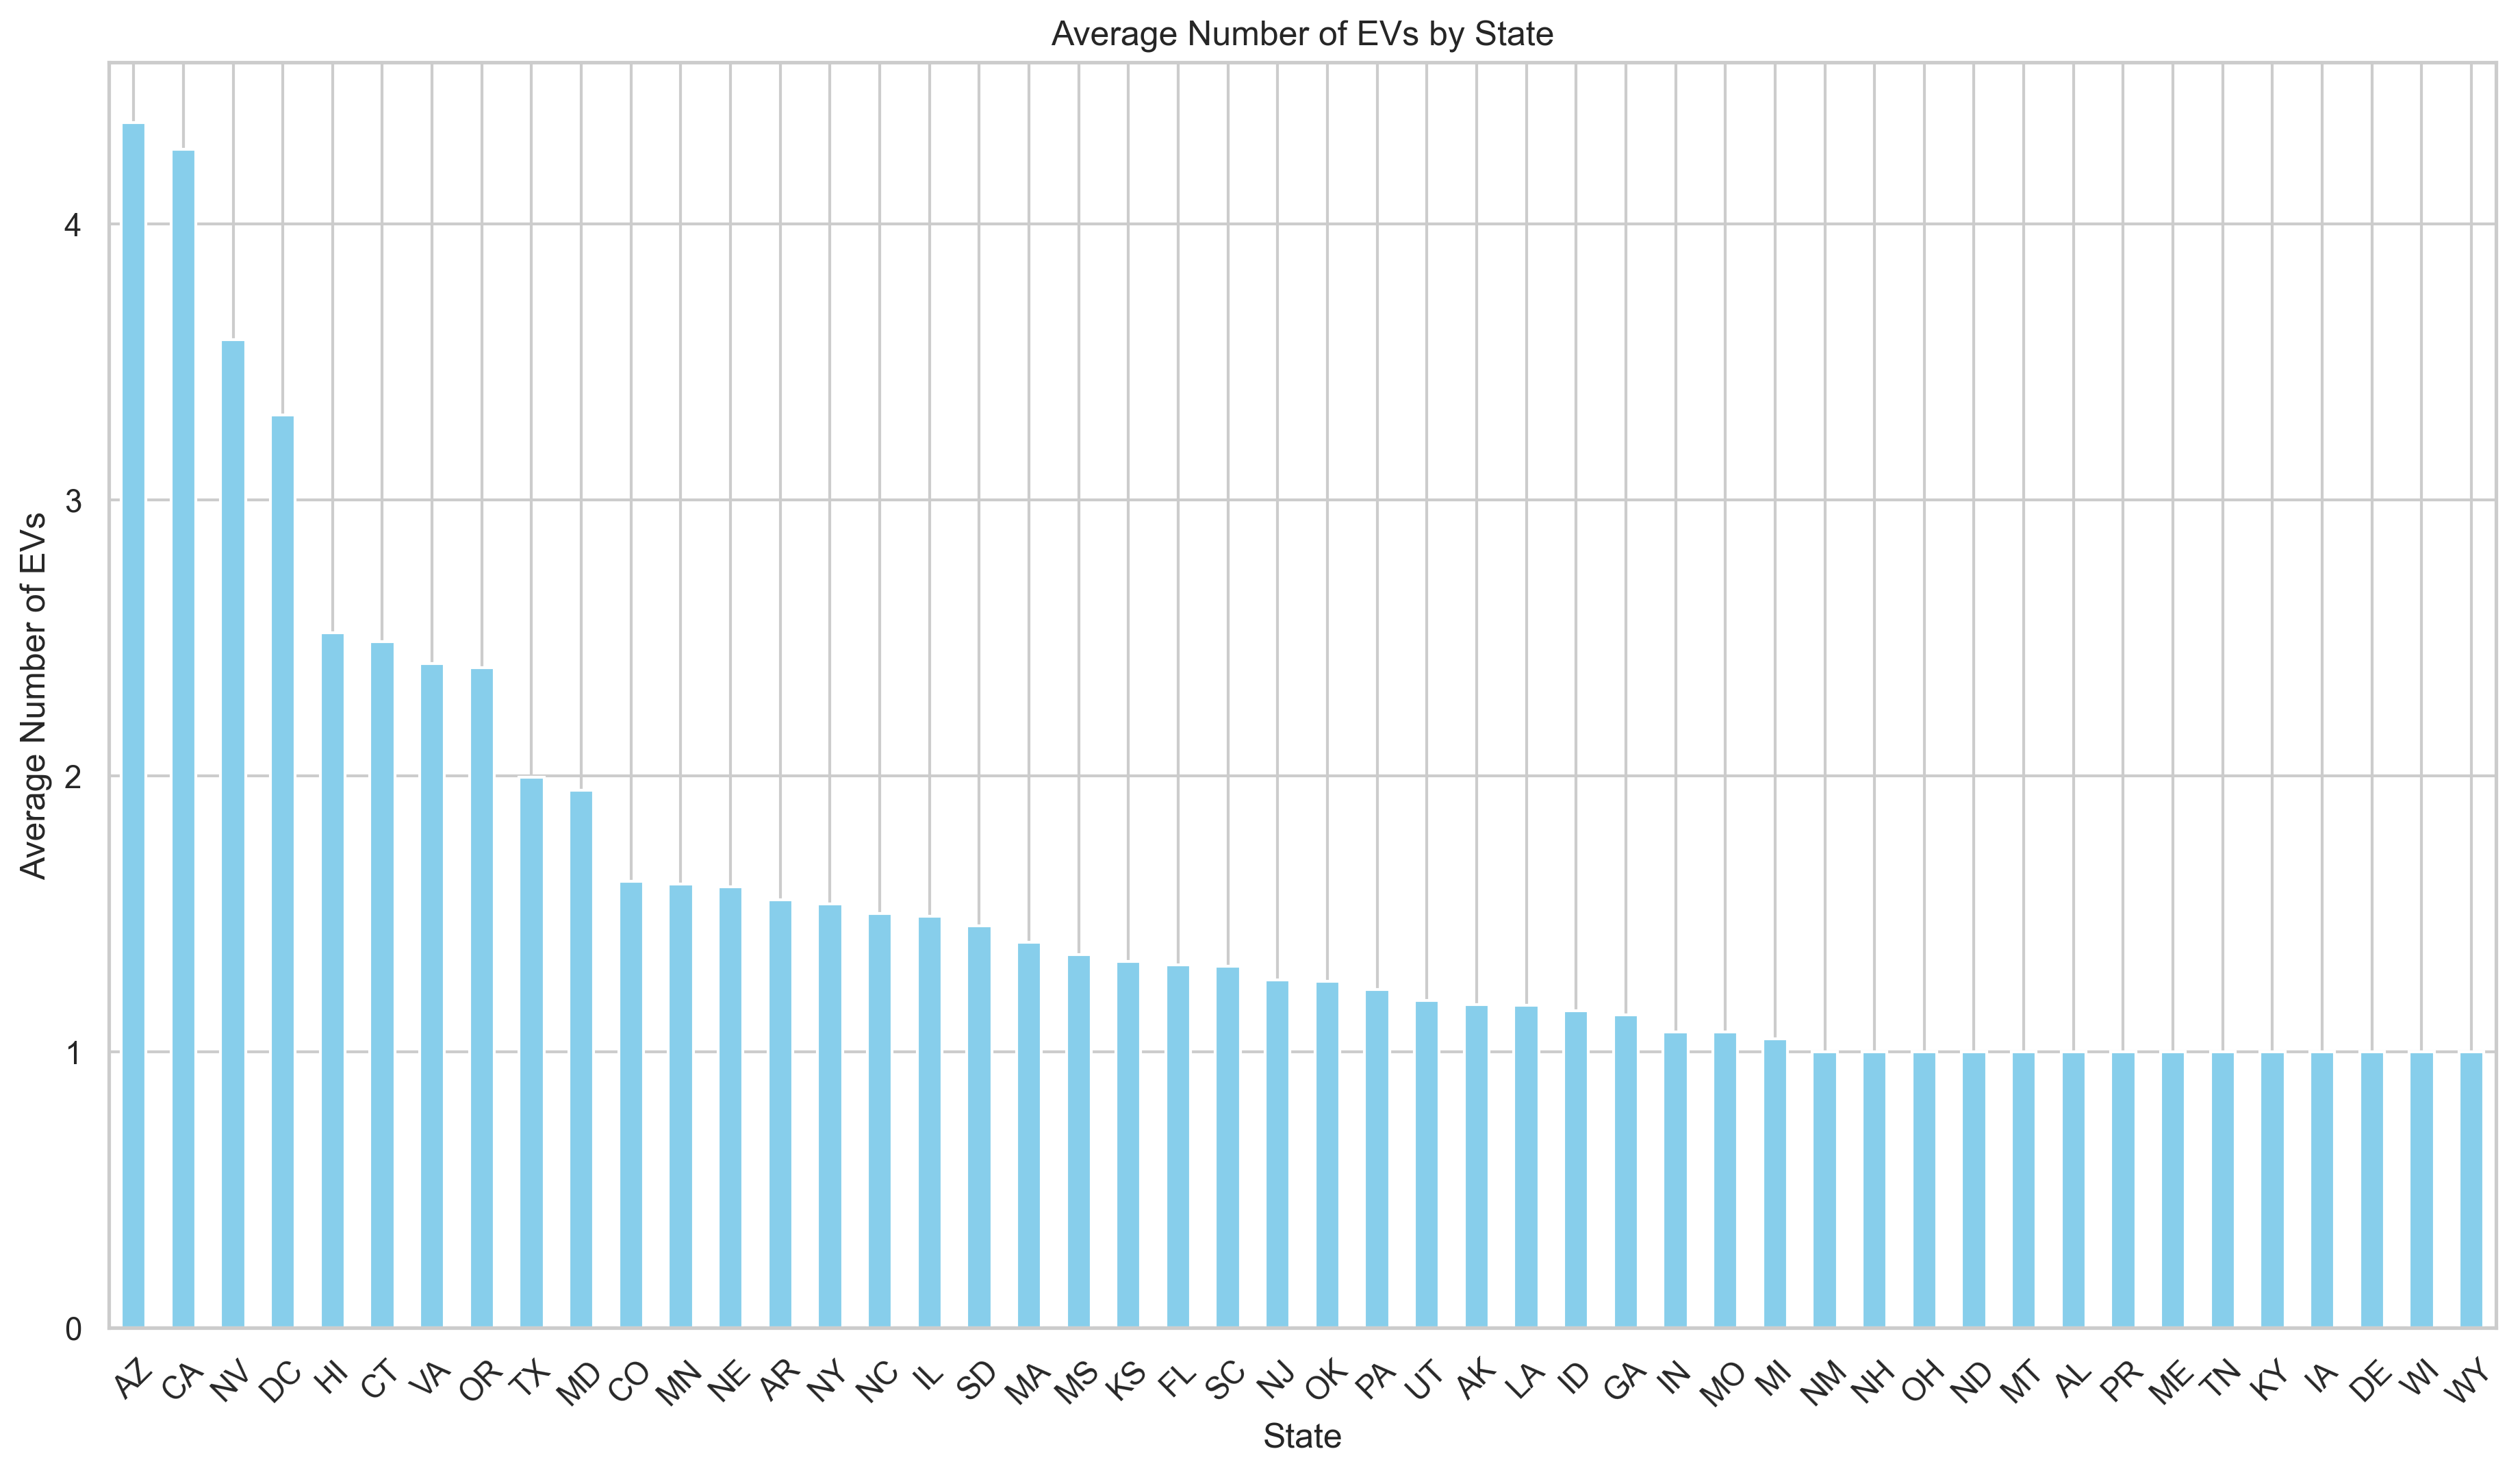
\includegraphics{SummaryPaper_FinalProject_T1_files/figure-pdf/cell-16-output-1.png}

}

\end{figure}

\textbf{Observation:} Arizona leads the way in average EVs per state,
indicating high adoption rates, which could be attributed to favourable
incentives or infrastructure. The descending order contrasts sharply
with states at the opposite end of the spectrum, where adoption is
clearly lower.

\begin{Shaded}
\begin{Highlighting}[]
\ImportTok{import}\NormalTok{ warnings}
\NormalTok{warnings.filterwarnings(}\StringTok{"ignore"}\NormalTok{)}
\NormalTok{bevs\_by\_region }\OperatorTok{=}\NormalTok{ df.groupby(}\StringTok{\textquotesingle{}Region\textquotesingle{}}\NormalTok{)[}\StringTok{\textquotesingle{}Battery Electric Vehicles (BEVs)\textquotesingle{}}\NormalTok{].}\BuiltInTok{sum}\NormalTok{()}
\NormalTok{phevs\_by\_region }\OperatorTok{=}\NormalTok{ df.groupby(}\StringTok{\textquotesingle{}Region\textquotesingle{}}\NormalTok{)[}\StringTok{\textquotesingle{}Plug{-}In Hybrid Electric Vehicles (PHEVs)\textquotesingle{}}\NormalTok{].}\BuiltInTok{sum}\NormalTok{()}

\CommentTok{\# Stacking BEVs and PHEVs}
\NormalTok{plt.figure(figsize}\OperatorTok{=}\NormalTok{(}\DecValTok{10}\NormalTok{, }\DecValTok{6}\NormalTok{))}
\NormalTok{plt.bar(bevs\_by\_region.index, bevs\_by\_region, label}\OperatorTok{=}\StringTok{\textquotesingle{}BEVs\textquotesingle{}}\NormalTok{, color}\OperatorTok{=}\StringTok{\textquotesingle{}blue\textquotesingle{}}\NormalTok{, alpha}\OperatorTok{=}\FloatTok{0.7}\NormalTok{)}
\NormalTok{plt.bar(phevs\_by\_region.index, phevs\_by\_region, bottom}\OperatorTok{=}\NormalTok{bevs\_by\_region, label}\OperatorTok{=}\StringTok{\textquotesingle{}PHEVs\textquotesingle{}}\NormalTok{, color}\OperatorTok{=}\StringTok{\textquotesingle{}orange\textquotesingle{}}\NormalTok{, alpha}\OperatorTok{=}\FloatTok{0.7}\NormalTok{)}
\NormalTok{plt.title(}\StringTok{\textquotesingle{}Comparison of BEVs and PHEVs by Region\textquotesingle{}}\NormalTok{)}
\NormalTok{plt.xlabel(}\StringTok{\textquotesingle{}Region\textquotesingle{}}\NormalTok{)}
\NormalTok{plt.ylabel(}\StringTok{\textquotesingle{}Number of Vehicles\textquotesingle{}}\NormalTok{)}
\NormalTok{plt.legend()}
\NormalTok{plt.show()}
\end{Highlighting}
\end{Shaded}

\begin{figure}[H]

{\centering 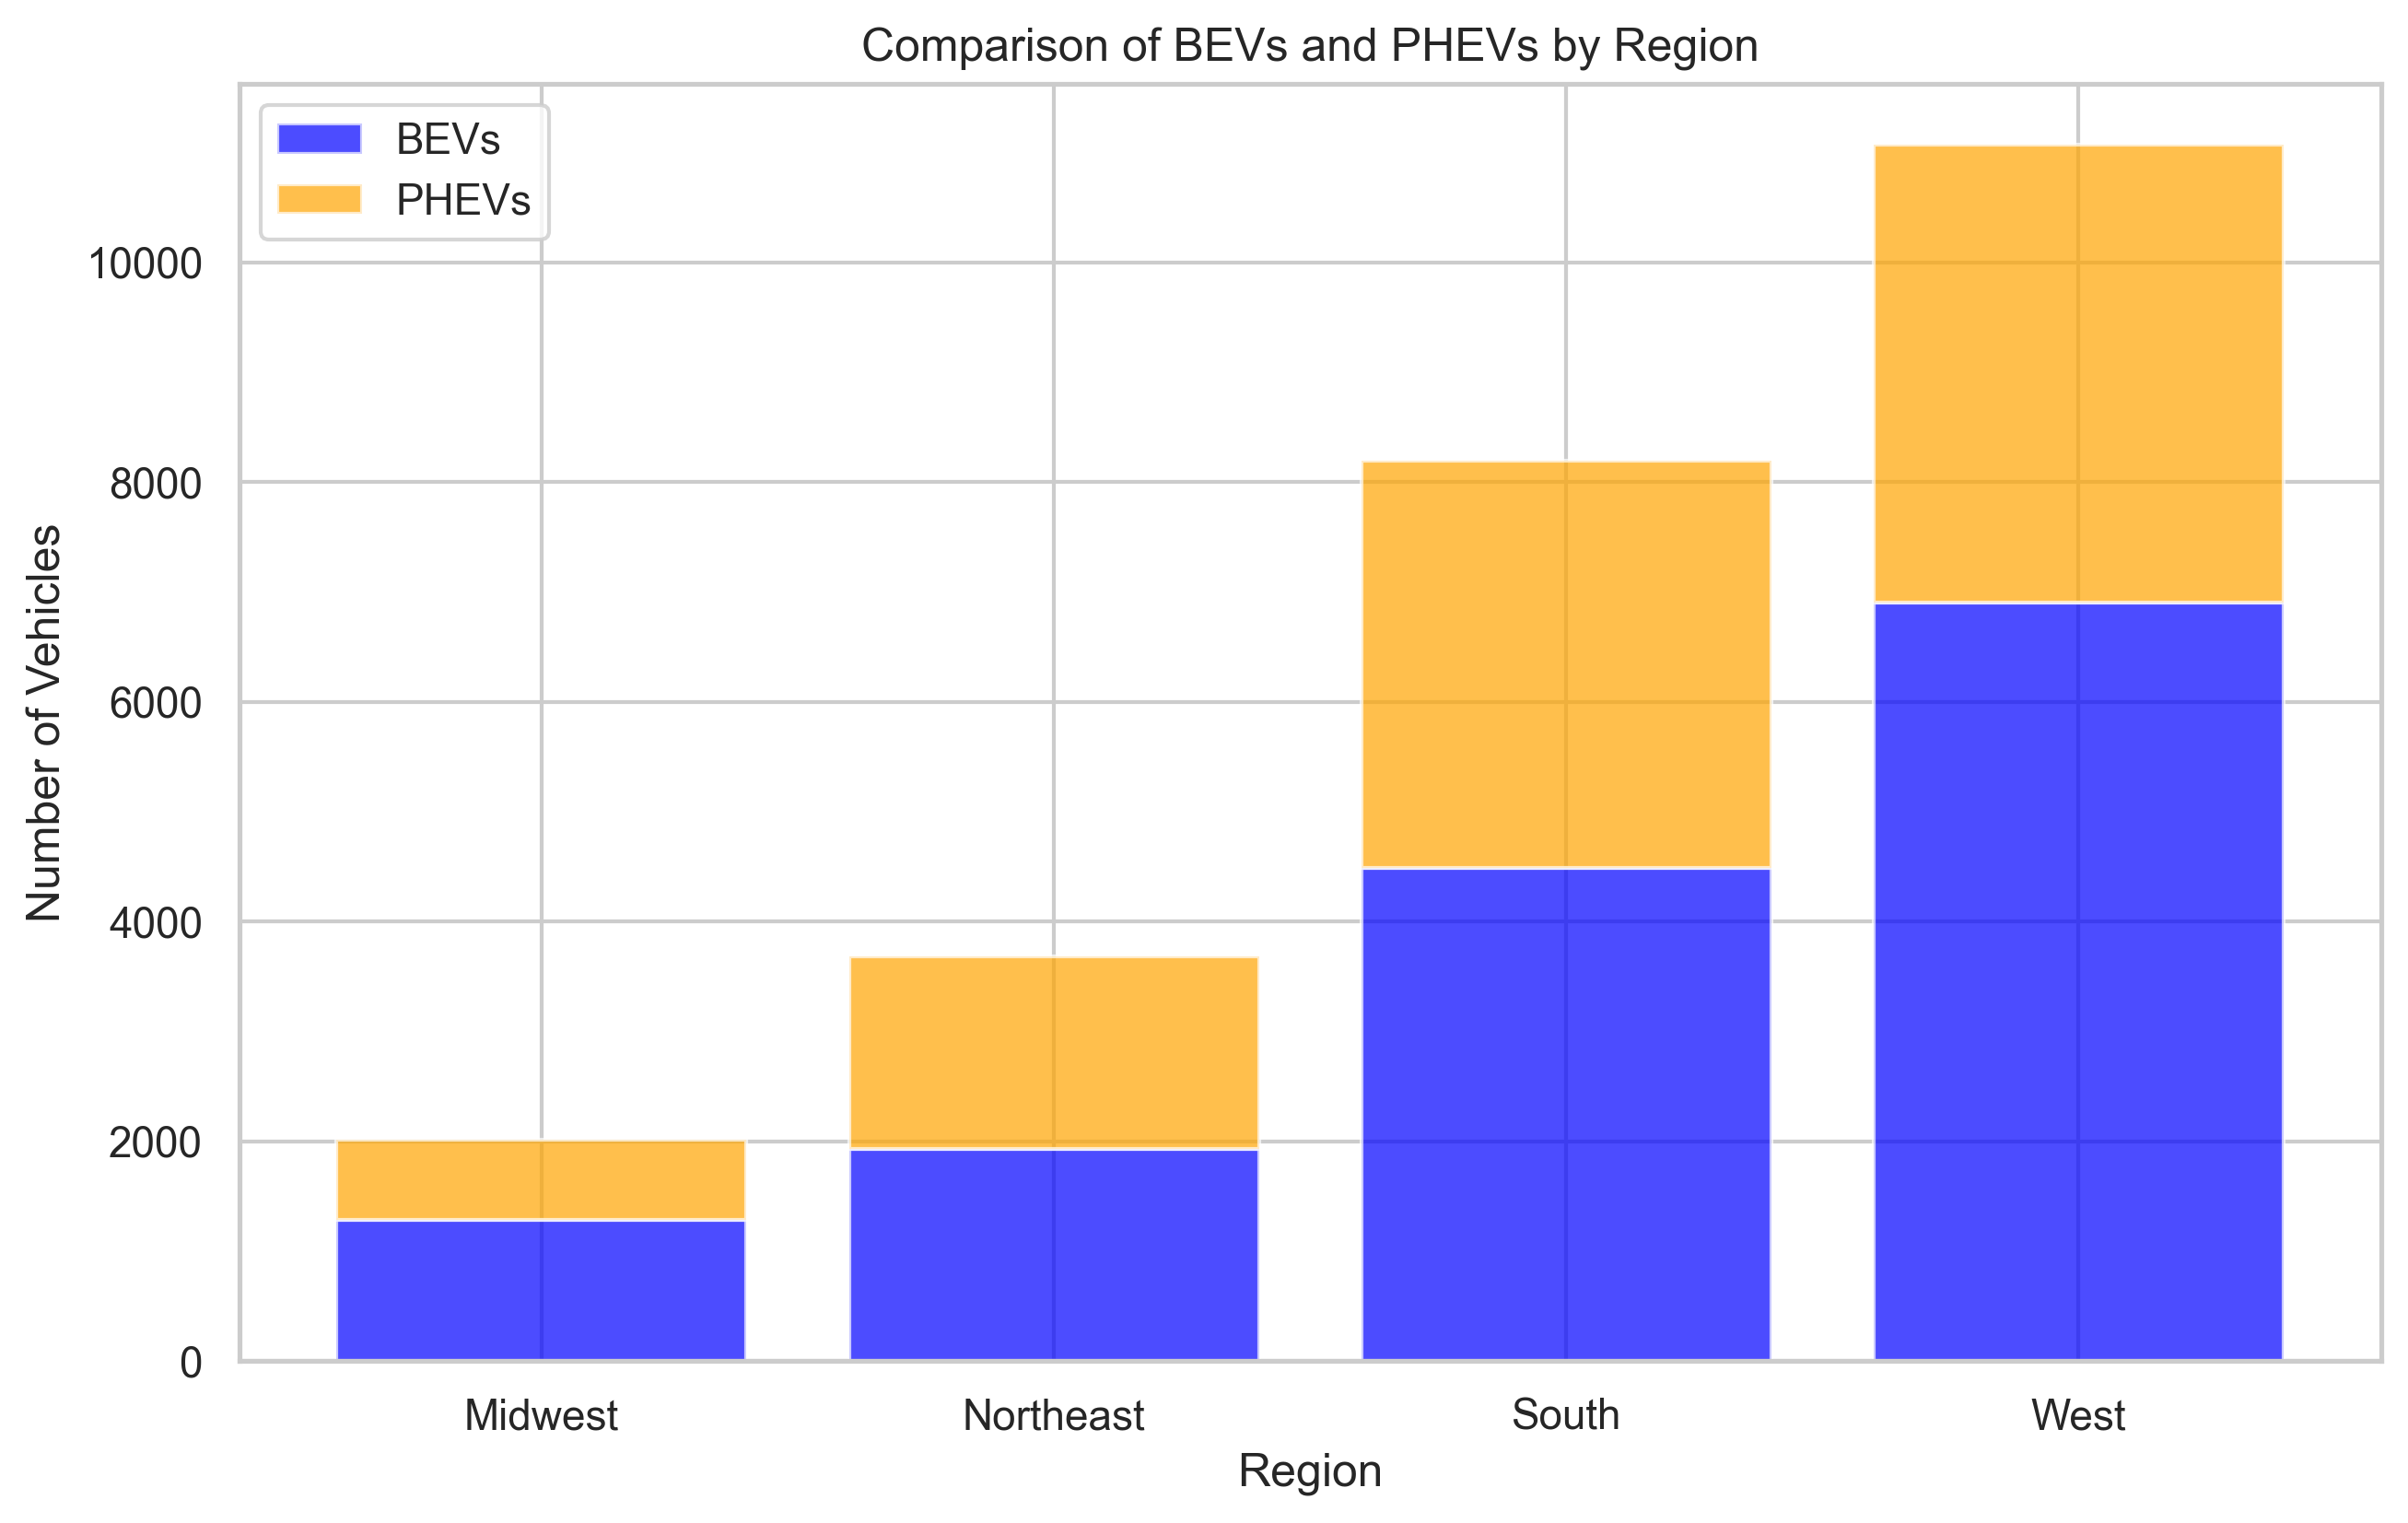
\includegraphics{SummaryPaper_FinalProject_T1_files/figure-pdf/cell-17-output-1.png}

}

\end{figure}

\textbf{Observation:} The West leads not only in total EV numbers, but
also in the preference for BEVs over PHEVs. The chart highlights
regional differences in vehicle type preferences, with the West
favouring all-electric vehicles.

\begin{Shaded}
\begin{Highlighting}[]
\ImportTok{import}\NormalTok{ warnings}
\NormalTok{warnings.filterwarnings(}\StringTok{"ignore"}\NormalTok{)}
\ImportTok{import}\NormalTok{ numpy }\ImportTok{as}\NormalTok{ np}
\CommentTok{\# Assuming df1 is already loaded and preprocessed as before}
\NormalTok{county\_region\_grouped }\OperatorTok{=}\NormalTok{ df.groupby([}\StringTok{\textquotesingle{}Region\textquotesingle{}}\NormalTok{, }\StringTok{\textquotesingle{}County\textquotesingle{}}\NormalTok{]).agg(\{}
    \StringTok{\textquotesingle{}Battery Electric Vehicles (BEVs)\textquotesingle{}}\NormalTok{: }\StringTok{\textquotesingle{}sum\textquotesingle{}}\NormalTok{, }
    \StringTok{\textquotesingle{}Plug{-}In Hybrid Electric Vehicles (PHEVs)\textquotesingle{}}\NormalTok{: }\StringTok{\textquotesingle{}sum\textquotesingle{}}
\NormalTok{\}).reset\_index()}

\CommentTok{\# Adding a total EVs column for sorting}
\NormalTok{county\_region\_grouped[}\StringTok{\textquotesingle{}Total EVs\textquotesingle{}}\NormalTok{] }\OperatorTok{=}\NormalTok{ county\_region\_grouped[}\StringTok{\textquotesingle{}Battery Electric Vehicles (BEVs)\textquotesingle{}}\NormalTok{] }\OperatorTok{+}\NormalTok{ county\_region\_grouped[}\StringTok{\textquotesingle{}Plug{-}In Hybrid Electric Vehicles (PHEVs)\textquotesingle{}}\NormalTok{]}

\CommentTok{\# Sorting to get the top 20 counties overall based on total EVs}
\NormalTok{top\_20\_counties\_overall }\OperatorTok{=}\NormalTok{ county\_region\_grouped.sort\_values(by}\OperatorTok{=}\StringTok{\textquotesingle{}Total EVs\textquotesingle{}}\NormalTok{, ascending}\OperatorTok{=}\VariableTok{False}\NormalTok{).head(}\DecValTok{20}\NormalTok{)}

\CommentTok{\# Extracting the unique regions from the top 20 counties}
\NormalTok{regions }\OperatorTok{=}\NormalTok{ top\_20\_counties\_overall[}\StringTok{\textquotesingle{}Region\textquotesingle{}}\NormalTok{].unique()}

\CommentTok{\# Assigning different colors for each region using NumPy}
\NormalTok{colors }\OperatorTok{=}\NormalTok{ plt.cm.viridis(np.linspace(}\DecValTok{0}\NormalTok{, }\DecValTok{1}\NormalTok{, }\BuiltInTok{len}\NormalTok{(regions)))}
\NormalTok{region\_colors }\OperatorTok{=}\NormalTok{ \{region: color }\ControlFlowTok{for}\NormalTok{ region, color }\KeywordTok{in} \BuiltInTok{zip}\NormalTok{(regions, colors)\}}

\CommentTok{\# Creating the bar plot for the top 20 counties, colored by their region}
\NormalTok{plt.figure(figsize}\OperatorTok{=}\NormalTok{(}\DecValTok{15}\NormalTok{, }\DecValTok{8}\NormalTok{))}
\ControlFlowTok{for}\NormalTok{ \_, row }\KeywordTok{in}\NormalTok{ top\_20\_counties\_overall.iterrows():}
\NormalTok{    plt.bar(row[}\StringTok{\textquotesingle{}County\textquotesingle{}}\NormalTok{], row[}\StringTok{\textquotesingle{}Battery Electric Vehicles (BEVs)\textquotesingle{}}\NormalTok{], color}\OperatorTok{=}\NormalTok{region\_colors[row[}\StringTok{\textquotesingle{}Region\textquotesingle{}}\NormalTok{]], edgecolor}\OperatorTok{=}\StringTok{\textquotesingle{}white\textquotesingle{}}\NormalTok{)}
\NormalTok{    plt.bar(row[}\StringTok{\textquotesingle{}County\textquotesingle{}}\NormalTok{], row[}\StringTok{\textquotesingle{}Plug{-}In Hybrid Electric Vehicles (PHEVs)\textquotesingle{}}\NormalTok{], bottom}\OperatorTok{=}\NormalTok{row[}\StringTok{\textquotesingle{}Battery Electric Vehicles (BEVs)\textquotesingle{}}\NormalTok{], color}\OperatorTok{=}\NormalTok{region\_colors[row[}\StringTok{\textquotesingle{}Region\textquotesingle{}}\NormalTok{]], alpha}\OperatorTok{=}\FloatTok{0.5}\NormalTok{, edgecolor}\OperatorTok{=}\StringTok{\textquotesingle{}white\textquotesingle{}}\NormalTok{)}

\CommentTok{\# Creating a custom legend}
\NormalTok{legend\_patches }\OperatorTok{=}\NormalTok{ [mpatches.Patch(color}\OperatorTok{=}\NormalTok{color, label}\OperatorTok{=}\NormalTok{region) }\ControlFlowTok{for}\NormalTok{ region, color }\KeywordTok{in}\NormalTok{ region\_colors.items()]}
\NormalTok{plt.legend(handles}\OperatorTok{=}\NormalTok{legend\_patches, title}\OperatorTok{=}\StringTok{\textquotesingle{}Region\textquotesingle{}}\NormalTok{)}

\NormalTok{plt.title(}\StringTok{\textquotesingle{}Top 20 Counties in EV Adoption (BEVs and PHEVs) by Region\textquotesingle{}}\NormalTok{)}
\NormalTok{plt.xlabel(}\StringTok{\textquotesingle{}County\textquotesingle{}}\NormalTok{)}
\NormalTok{plt.ylabel(}\StringTok{\textquotesingle{}Number of Vehicles\textquotesingle{}}\NormalTok{)}
\NormalTok{plt.xticks(rotation}\OperatorTok{=}\DecValTok{45}\NormalTok{)}
\NormalTok{plt.show()}
\end{Highlighting}
\end{Shaded}

\begin{figure}[H]

{\centering 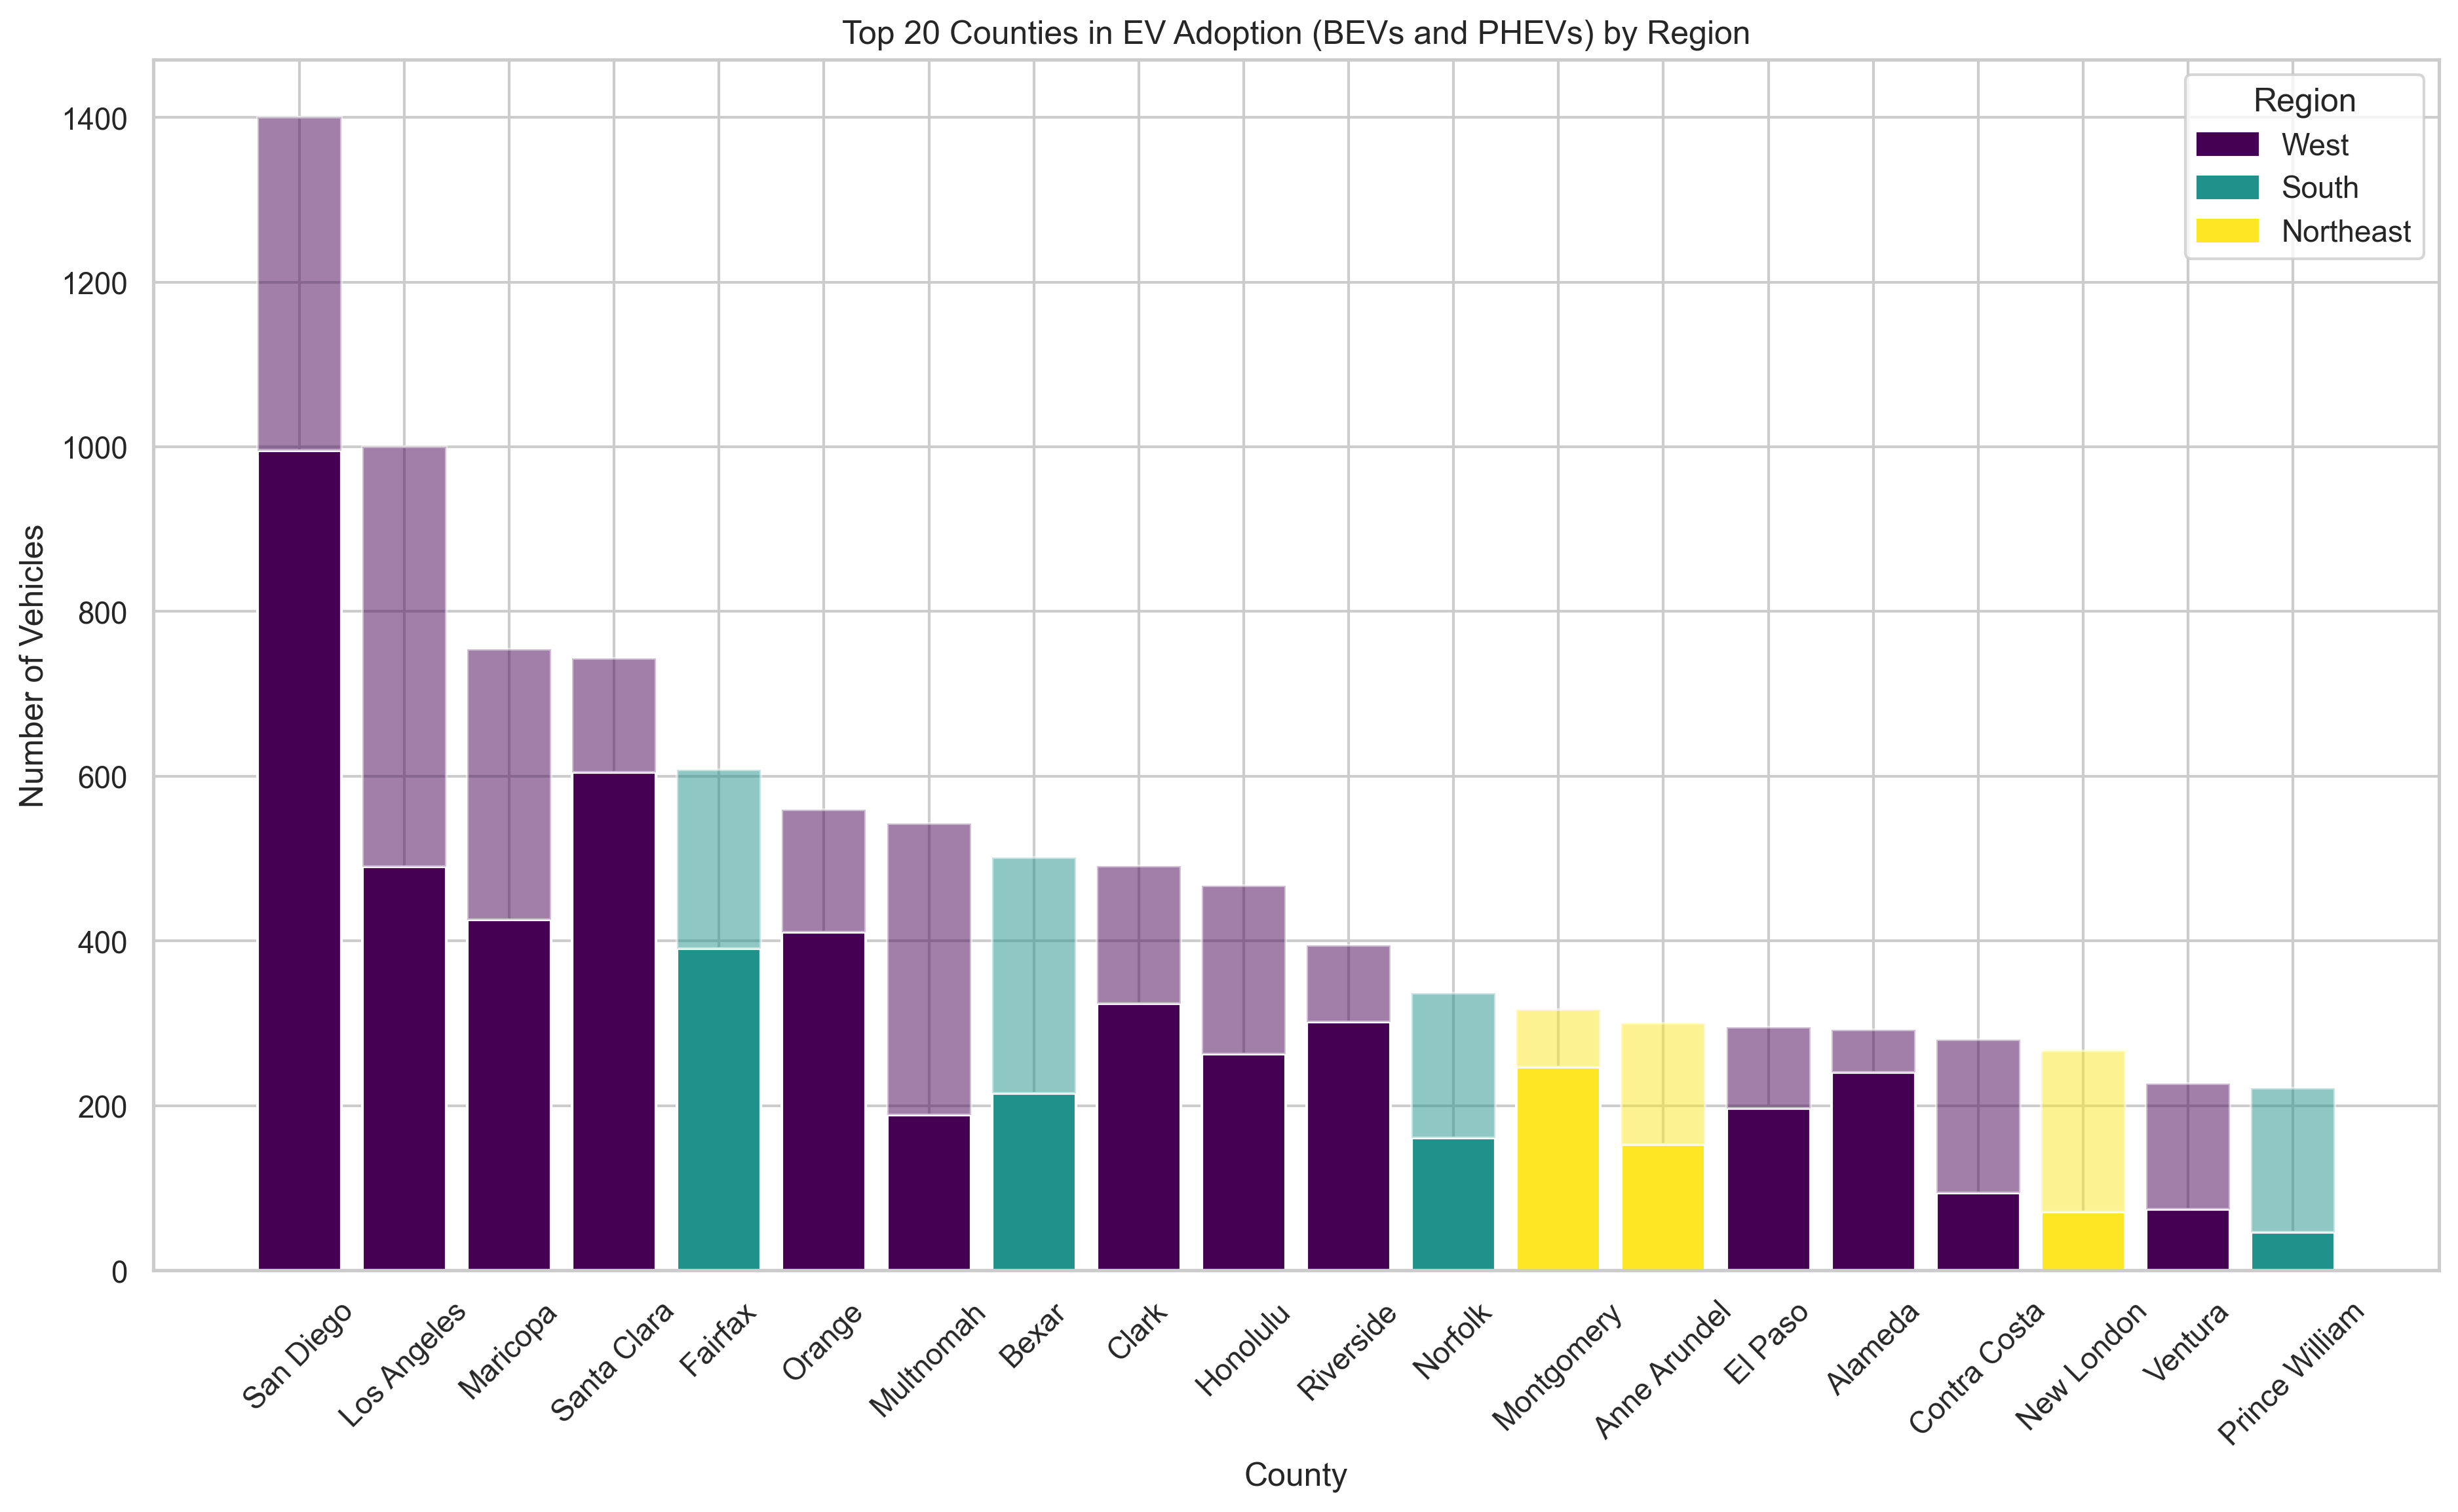
\includegraphics{SummaryPaper_FinalProject_T1_files/figure-pdf/cell-18-output-1.png}

}

\end{figure}

\textbf{Observation:} In terms of total EV adoption, San Diego and Los
Angeles counties have a significant lead. The graphic depicts regional
EV hotspots, with the West, particularly California, dominating the
chart, reflecting regional policy success and consumer preference for
electric mobility.

\hypertarget{hypothesis-testing}{%
\section{HYPOTHESIS TESTING}\label{hypothesis-testing}}

\hypertarget{test-1}{%
\subsection{TEST 1}\label{test-1}}

\hypertarget{anova-test}{%
\subsubsection{ANOVA test}\label{anova-test}}

\hypertarget{is-there-a-significant-difference-in-the-average-number-of-evs-among-different-years-comparing-2017-2019-and-2021}{%
\paragraph{Is there a significant difference in the average number of
EVs among different years (comparing 2017, 2019, and
2021)?}\label{is-there-a-significant-difference-in-the-average-number-of-evs-among-different-years-comparing-2017-2019-and-2021}}

\begin{Shaded}
\begin{Highlighting}[]
\ImportTok{import}\NormalTok{ warnings}
\NormalTok{warnings.filterwarnings(}\StringTok{"ignore"}\NormalTok{)}

\CommentTok{\#Null Hypothesis (H0): There is no significant difference in the average number of EVs among the years 2017, 2019, and 2021. }
\CommentTok{\#This implies that any observed differences are due to random chance.}
\CommentTok{\#Alternative Hypothesis (H1): There is a significant difference in the average number of EVs among these years, indicating that changes over the years are not just random variations.}

\ImportTok{from}\NormalTok{ scipy.stats }\ImportTok{import}\NormalTok{ f\_oneway}
\ImportTok{import}\NormalTok{ pandas }\ImportTok{as}\NormalTok{ pd}

\NormalTok{df\_years }\OperatorTok{=}\NormalTok{ df[df[}\StringTok{\textquotesingle{}Year\textquotesingle{}}\NormalTok{].isin([}\DecValTok{2017}\NormalTok{, }\DecValTok{2019}\NormalTok{, }\DecValTok{2021}\NormalTok{])]}

\CommentTok{\# Extract the EV totals for each of these years}
\NormalTok{data\_2017 }\OperatorTok{=}\NormalTok{ df\_years[df\_years[}\StringTok{\textquotesingle{}Year\textquotesingle{}}\NormalTok{] }\OperatorTok{==} \DecValTok{2017}\NormalTok{][}\StringTok{\textquotesingle{}Electric Vehicle (EV) Total\textquotesingle{}}\NormalTok{]}
\NormalTok{data\_2019 }\OperatorTok{=}\NormalTok{ df\_years[df\_years[}\StringTok{\textquotesingle{}Year\textquotesingle{}}\NormalTok{] }\OperatorTok{==} \DecValTok{2019}\NormalTok{][}\StringTok{\textquotesingle{}Electric Vehicle (EV) Total\textquotesingle{}}\NormalTok{]}
\NormalTok{data\_2021 }\OperatorTok{=}\NormalTok{ df\_years[df\_years[}\StringTok{\textquotesingle{}Year\textquotesingle{}}\NormalTok{] }\OperatorTok{==} \DecValTok{2021}\NormalTok{][}\StringTok{\textquotesingle{}Electric Vehicle (EV) Total\textquotesingle{}}\NormalTok{]}

\CommentTok{\# Perform ANOVA test}
\NormalTok{anova\_result }\OperatorTok{=}\NormalTok{ f\_oneway(data\_2017, data\_2019, data\_2021)}

\CommentTok{\# Output the result}
\BuiltInTok{print}\NormalTok{(anova\_result)}
\end{Highlighting}
\end{Shaded}

\begin{verbatim}
F_onewayResult(statistic=25.423195756856018, pvalue=1.0250901376196195e-11)
\end{verbatim}

\textbf{Observation:} The ANOVA test reveals a highly significant
difference in the average number of EVs between 2017, 2019, and 2021
(p-value 0.00001). The statistic shows a statistically significant
change in EV numbers over these years, implying that the factors
influencing EV adoption have evolved, resulting in fluctuations in
annual EV adoption rates. This finding calls for more research into the
specific annual factors influencing these variations, such as policy
changes, technological advancements, or economic incentives.

\hypertarget{test-2}{%
\subsection{TEST 2}\label{test-2}}

\hypertarget{chi-square-test}{%
\subsubsection{CHI-SQUARE test}\label{chi-square-test}}

\hypertarget{smart-question-2-is-there-a-statistically-significant-association-between-geographic-regions-and-the-primary-use-categories-of-electric-vehicles}{%
\paragraph{SMART QUESTION 2: Is there a statistically significant
association between geographic regions and the primary use categories of
electric
vehicles?}\label{smart-question-2-is-there-a-statistically-significant-association-between-geographic-regions-and-the-primary-use-categories-of-electric-vehicles}}

\begin{Shaded}
\begin{Highlighting}[]
\ImportTok{import}\NormalTok{ warnings}
\NormalTok{warnings.filterwarnings(}\StringTok{"ignore"}\NormalTok{)}
\ImportTok{import}\NormalTok{ pandas }\ImportTok{as}\NormalTok{ pd}
\ImportTok{from}\NormalTok{ scipy.stats }\ImportTok{import}\NormalTok{ chi2\_contingency}

\CommentTok{\#Null Hypothesis (H0): There is no association between the region and the vehicle primary use category in terms of EV adoption.}
\CommentTok{\#This means any observed association is due to random chance.}
\CommentTok{\#Alternative Hypothesis (H1): There is an association between the region and the vehicle primary use  category in terms of EV adoption. }
\CommentTok{\#This means the observed association is not due to random chance.}

\NormalTok{contingency\_table }\OperatorTok{=}\NormalTok{ pd.crosstab(df[}\StringTok{\textquotesingle{}Region\textquotesingle{}}\NormalTok{], df[}\StringTok{\textquotesingle{}Vehicle Primary Use\textquotesingle{}}\NormalTok{])}

\NormalTok{chi2, p\_value, dof, expected }\OperatorTok{=}\NormalTok{ chi2\_contingency(contingency\_table)}

\CommentTok{\# Output the results}
\BuiltInTok{print}\NormalTok{(}\StringTok{"Chi{-}square statistic:"}\NormalTok{, chi2)}
\BuiltInTok{print}\NormalTok{(}\StringTok{"p{-}value:"}\NormalTok{, p\_value)}
\BuiltInTok{print}\NormalTok{(}\StringTok{"}\CharTok{\textbackslash{}n}\StringTok{Contingency Table:"}\NormalTok{)}
\BuiltInTok{print}\NormalTok{(contingency\_table)}
\end{Highlighting}
\end{Shaded}

\begin{verbatim}
Chi-square statistic: 19.06683791983831
p-value: 0.00026483531434350613

Contingency Table:
Vehicle Primary Use  Passenger  Truck
Region                               
Midwest                   1575     12
Northeast                 2302      0
South                     4921     12
West                      3724     15
\end{verbatim}

\textbf{Conclusion for SMART Q2:}

The chi-square test reveals a significant relationship between
geographic regions and electric vehicle primary use categories (p-value
0.001). The contingency table reveals regional disparities, with the
South leading in passenger EVs and the West balancing passenger and
truck categories. This suggests regional differences in EV usage
patterns, which could be influenced by regional lifestyles,
infrastructure, or economic factors.

\hypertarget{test-3}{%
\subsection{TEST 3}\label{test-3}}

\hypertarget{t-test}{%
\subsubsection{T-Test}\label{t-test}}

\hypertarget{smart-question3-is-there-a-significant-difference-in-the-average-number-of-electric-vehicles-evs-between-the-top-5-counties-of-the-south-region-and-the-top-5-counties-of-the-northeast-region-in-the-united-states}{%
\paragraph{SMART QUESTION3: Is there a significant difference in the
average number of electric vehicles (EVs) between the top 5 counties of
the South region and the top 5 counties of the Northeast region in the
United
States?}\label{smart-question3-is-there-a-significant-difference-in-the-average-number-of-electric-vehicles-evs-between-the-top-5-counties-of-the-south-region-and-the-top-5-counties-of-the-northeast-region-in-the-united-states}}

\begin{Shaded}
\begin{Highlighting}[]
\ImportTok{import}\NormalTok{ warnings}
\NormalTok{warnings.filterwarnings(}\StringTok{"ignore"}\NormalTok{)}
\ImportTok{from}\NormalTok{ scipy.stats }\ImportTok{import}\NormalTok{ ttest\_ind}
\CommentTok{\#H0 The mean number of EVs in the top 5 counties of the South region is equal to or greater than the mean number of EVs in the top 5 counties of the Northeast region. }
\CommentTok{\#H1: The mean number of EVs in the top 5 counties of the South region is less than the mean number of EVs in the top 5 counties of the Northeast region.}

\NormalTok{data\_2023\_northeast }\OperatorTok{=}\NormalTok{ df[(df[}\StringTok{\textquotesingle{}Year\textquotesingle{}}\NormalTok{] }\OperatorTok{==} \DecValTok{2023}\NormalTok{) }\OperatorTok{\&}\NormalTok{ (df[}\StringTok{\textquotesingle{}Region\textquotesingle{}}\NormalTok{] }\OperatorTok{==} \StringTok{\textquotesingle{}Northeast\textquotesingle{}}\NormalTok{)]}
\NormalTok{county\_ev\_totals\_northeast }\OperatorTok{=}\NormalTok{ data\_2023\_northeast.groupby(}\StringTok{\textquotesingle{}County\textquotesingle{}}\NormalTok{)[}\StringTok{\textquotesingle{}Electric Vehicle (EV) Total\textquotesingle{}}\NormalTok{].}\BuiltInTok{sum}\NormalTok{()}
\NormalTok{top5\_counties\_northeast }\OperatorTok{=}\NormalTok{ county\_ev\_totals\_northeast.sort\_values(ascending}\OperatorTok{=}\VariableTok{False}\NormalTok{).head(}\DecValTok{5}\NormalTok{)}
\NormalTok{data\_2023\_south }\OperatorTok{=}\NormalTok{ df[(df[}\StringTok{\textquotesingle{}Year\textquotesingle{}}\NormalTok{] }\OperatorTok{==} \DecValTok{2023}\NormalTok{) }\OperatorTok{\&}\NormalTok{ (df[}\StringTok{\textquotesingle{}Region\textquotesingle{}}\NormalTok{] }\OperatorTok{==} \StringTok{\textquotesingle{}South\textquotesingle{}}\NormalTok{)]}
\NormalTok{county\_ev\_totals }\OperatorTok{=}\NormalTok{ data\_2023\_south.groupby(}\StringTok{\textquotesingle{}County\textquotesingle{}}\NormalTok{)[}\StringTok{\textquotesingle{}Electric Vehicle (EV) Total\textquotesingle{}}\NormalTok{].}\BuiltInTok{sum}\NormalTok{()}

\NormalTok{top5\_counties }\OperatorTok{=}\NormalTok{ county\_ev\_totals.sort\_values(ascending}\OperatorTok{=}\VariableTok{False}\NormalTok{).head(}\DecValTok{5}\NormalTok{)}


\NormalTok{mean\_south }\OperatorTok{=}\NormalTok{ top5\_counties.mean()}
\NormalTok{mean\_northeast }\OperatorTok{=}\NormalTok{ top5\_counties\_northeast.mean()}

\CommentTok{\# Perform a t{-}test}
\CommentTok{\# Since we are doing a one{-}tailed test, we need to divide the p{-}value by 2}
\NormalTok{t\_stat, p\_value }\OperatorTok{=}\NormalTok{ ttest\_ind(top5\_counties, top5\_counties\_northeast, equal\_var}\OperatorTok{=}\VariableTok{False}\NormalTok{)}
\NormalTok{p\_value\_one\_tailed }\OperatorTok{=}\NormalTok{ p\_value }\OperatorTok{/} \DecValTok{2}

\NormalTok{mean\_south, mean\_northeast, t\_stat, p\_value\_one\_tailed }

\BuiltInTok{print}\NormalTok{(}\StringTok{"t{-}stat:"}\NormalTok{,t\_stat)}
\BuiltInTok{print}\NormalTok{(}\StringTok{"p\_value"}\NormalTok{,p\_value\_one\_tailed)}
\end{Highlighting}
\end{Shaded}

\begin{verbatim}
t-stat: 0.07371697182914644
p_value 0.4715510434929737
\end{verbatim}

\textbf{Conclusion for SMART Q3:}

The p-value is much higher than the commonly used significance level of
0.05 so we failed to reject null hypothesis so we conclude that the mean
number of EVs in the top 5 counties of the South region is less than
that in the top 5 counties of the Northeast region. We have seen that
the trend of EV adoption in each region in that we have seen Northeast
have higher adoption than south from 2022 to 2023 we are using the above
test to check northeast adoption or increase of ev not due to top5
counties but rather average of all counties from the t-test the top5
south region having highest EV adoption but overall it decreased

\hypertarget{modelling}{%
\section{MODELLING}\label{modelling}}

\hypertarget{ols-regression}{%
\subsection{OLS Regression}\label{ols-regression}}

\hypertarget{smart-question-4-is-there-a-relationship-between-the-year-and-total-vehicle-count-in-predicting-regional-ev-adoption}{%
\subsubsection{SMART QUESTION 4: Is there a relationship between the
year and total vehicle count in predicting regional EV
adoption?}\label{smart-question-4-is-there-a-relationship-between-the-year-and-total-vehicle-count-in-predicting-regional-ev-adoption}}

\begin{Shaded}
\begin{Highlighting}[]
\ImportTok{import}\NormalTok{ warnings}
\NormalTok{warnings.filterwarnings(}\StringTok{"ignore"}\NormalTok{)}
\ImportTok{import}\NormalTok{ statsmodels.api }\ImportTok{as}\NormalTok{ sm}

\CommentTok{\# Preparing the data for linear regression}
\CommentTok{\# \textquotesingle{}Year\textquotesingle{} and \textquotesingle{}Total Vehicles\textquotesingle{} will be our independent variables (predictors)}
\CommentTok{\# \textquotesingle{}Electric Vehicle (EV) Total\textquotesingle{} is the dependent variable (target)}

\NormalTok{X }\OperatorTok{=}\NormalTok{ df[[}\StringTok{\textquotesingle{}Year\textquotesingle{}}\NormalTok{, }\StringTok{\textquotesingle{}Total Vehicles\textquotesingle{}}\NormalTok{]]  }\CommentTok{\# Independent variables}
\NormalTok{y }\OperatorTok{=}\NormalTok{ df[}\StringTok{\textquotesingle{}Electric Vehicle (EV) Total\textquotesingle{}}\NormalTok{]  }\CommentTok{\# Dependent variable}

\CommentTok{\# Adding a constant to the model (intercept)}
\NormalTok{X }\OperatorTok{=}\NormalTok{ sm.add\_constant(X)}

\CommentTok{\# Building the linear regression model}
\NormalTok{model }\OperatorTok{=}\NormalTok{ sm.OLS(y, X).fit()}

\CommentTok{\# Getting the summary of the regression}
\NormalTok{model\_summary }\OperatorTok{=}\NormalTok{ model.summary()}

\CommentTok{\# Print the summary}
\BuiltInTok{print}\NormalTok{(model\_summary)}
\end{Highlighting}
\end{Shaded}

\begin{verbatim}
                                 OLS Regression Results                                
=======================================================================================
Dep. Variable:     Electric Vehicle (EV) Total   R-squared:                       0.591
Model:                                     OLS   Adj. R-squared:                  0.591
Method:                          Least Squares   F-statistic:                     9158.
Date:                         Tue, 19 Dec 2023   Prob (F-statistic):               0.00
Time:                                 17:40:55   Log-Likelihood:                -23297.
No. Observations:                        12688   AIC:                         4.660e+04
Df Residuals:                            12685   BIC:                         4.662e+04
Df Model:                                    2                                         
Covariance Type:                     nonrobust                                         
==================================================================================
                     coef    std err          t      P>|t|      [0.025      0.975]
----------------------------------------------------------------------------------
const           -495.3557     14.768    -33.543      0.000    -524.302    -466.409
Year               0.2457      0.007     33.611      0.000       0.231       0.260
Total Vehicles     0.0065   4.85e-05    134.544      0.000       0.006       0.007
==============================================================================
Omnibus:                     5488.968   Durbin-Watson:                   2.000
Prob(Omnibus):                  0.000   Jarque-Bera (JB):           181296.233
Skew:                           1.440   Prob(JB):                         0.00
Kurtosis:                      21.293   Cond. No.                     2.22e+06
==============================================================================

Notes:
[1] Standard Errors assume that the covariance matrix of the errors is correctly specified.
[2] The condition number is large, 2.22e+06. This might indicate that there are
strong multicollinearity or other numerical problems.
\end{verbatim}

\textbf{Conclusion for SMART Q4:}

With an R-squared of 0.591, the OLS regression model demonstrates a
significant relationship between the year, total vehicle count, and
regional EV adoption. This means that the model accounts for
approximately 59\% of the variation in EV adoption. The year and total
vehicle count are significant predictors (p 0.0001), indicating that
temporal changes and vehicle availability play a role. The high
condition number, on the other hand, indicates the possibility of
multicollinearity, which may affect the reliability of the regression
coefficients. The model emphasises the significance of time trends and
vehicle accessibility in influencing regional EV adoption.

\hypertarget{logisticregression}{%
\subsection{LogisticRegression}\label{logisticregression}}

\hypertarget{smart-q5-can-demographic-and-regional-factors-such-as-year-state-and-region-effectively-predict-the-likelihood-of-a-county-having-high-electric-vehicle-adoption-rates}{%
\subsubsection{SMART Q5: Can demographic and regional factors, such as
year, state, and region, effectively predict the likelihood of a county
having high electric vehicle adoption
rates?}\label{smart-q5-can-demographic-and-regional-factors-such-as-year-state-and-region-effectively-predict-the-likelihood-of-a-county-having-high-electric-vehicle-adoption-rates}}

\textbf{Task:}

Predict whether a county has a high or low adoption of electric vehicles
based on the provided features.

\textbf{Target Variable:}

Create a binary target variable (e.g., ``High EV Adoption'' vs.~``Low EV
Adoption'') based on a threshold of Percent Electric Vehicles. Logistic
Regression: Use logistic regression to model the likelihood of high EV
adoption based on the other features.

\begin{Shaded}
\begin{Highlighting}[]
\ImportTok{import}\NormalTok{ warnings}
\NormalTok{warnings.filterwarnings(}\StringTok{"ignore"}\NormalTok{)}



\ImportTok{import}\NormalTok{ pandas }\ImportTok{as}\NormalTok{ pd}
\ImportTok{from}\NormalTok{ sklearn.linear\_model }\ImportTok{import}\NormalTok{ LogisticRegression}
\ImportTok{from}\NormalTok{ sklearn.model\_selection }\ImportTok{import}\NormalTok{ train\_test\_split}
\ImportTok{from}\NormalTok{ sklearn.preprocessing }\ImportTok{import}\NormalTok{ StandardScaler}

\CommentTok{\# Define the threshold for high vs. low EV adoption (you can adjust this threshold)}
\NormalTok{threshold }\OperatorTok{=} \FloatTok{5.0}  \CommentTok{\# For example, counties with \textgreater{}5\% adoption are considered "high" adoption}

\CommentTok{\# Create a binary target variable based on the threshold}
\NormalTok{df[}\StringTok{\textquotesingle{}HighEVAdoption\textquotesingle{}}\NormalTok{] }\OperatorTok{=}\NormalTok{ (df[}\StringTok{\textquotesingle{}Percent Electric Vehicles\textquotesingle{}}\NormalTok{] }\OperatorTok{\textgreater{}}\NormalTok{ threshold).astype(}\BuiltInTok{int}\NormalTok{)}

\CommentTok{\# Define the predictors (features)}
\NormalTok{X }\OperatorTok{=}\NormalTok{ df[[}\StringTok{\textquotesingle{}Year\textquotesingle{}}\NormalTok{, }\StringTok{\textquotesingle{}Electric Vehicle (EV) Total\textquotesingle{}}\NormalTok{, }\StringTok{\textquotesingle{}State\textquotesingle{}}\NormalTok{, }\StringTok{\textquotesingle{}Region\textquotesingle{}}\NormalTok{]]}

\CommentTok{\# Define the target variable}
\NormalTok{y }\OperatorTok{=}\NormalTok{ df[}\StringTok{\textquotesingle{}HighEVAdoption\textquotesingle{}}\NormalTok{]}

\CommentTok{\# Perform one{-}hot encoding for the categorical columns}
\NormalTok{X }\OperatorTok{=}\NormalTok{ pd.get\_dummies(X, columns}\OperatorTok{=}\NormalTok{[}\StringTok{\textquotesingle{}State\textquotesingle{}}\NormalTok{, }\StringTok{\textquotesingle{}Region\textquotesingle{}}\NormalTok{], drop\_first}\OperatorTok{=}\VariableTok{True}\NormalTok{)}

\CommentTok{\# Split the dataset into training and testing sets}
\NormalTok{X\_train, X\_test, y\_train, y\_test }\OperatorTok{=}\NormalTok{ train\_test\_split(X, y, test\_size}\OperatorTok{=}\FloatTok{0.2}\NormalTok{, random\_state}\OperatorTok{=}\DecValTok{42}\NormalTok{)}

\CommentTok{\# Standardize the features}
\NormalTok{scaler }\OperatorTok{=}\NormalTok{ StandardScaler()}
\NormalTok{X\_train\_scaled }\OperatorTok{=}\NormalTok{ scaler.fit\_transform(X\_train)}
\NormalTok{X\_test\_scaled }\OperatorTok{=}\NormalTok{ scaler.transform(X\_test)}

\CommentTok{\# Create and train the logistic regression model}
\NormalTok{model }\OperatorTok{=}\NormalTok{ LogisticRegression(random\_state}\OperatorTok{=}\DecValTok{42}\NormalTok{)}
\NormalTok{model.fit(X\_train\_scaled, y\_train)}

\CommentTok{\# Make predictions on the test set}
\NormalTok{y\_pred }\OperatorTok{=}\NormalTok{ model.predict(X\_test\_scaled)}

\CommentTok{\# Evaluate the model (you can print accuracy, precision, recall, etc., as needed)}
\ImportTok{from}\NormalTok{ sklearn.metrics }\ImportTok{import}\NormalTok{ accuracy\_score, classification\_report}
\BuiltInTok{print}\NormalTok{(}\StringTok{"Accuracy:"}\NormalTok{, accuracy\_score(y\_test, y\_pred))}
\BuiltInTok{print}\NormalTok{(}\StringTok{"Classification Report:"}\NormalTok{)}
\BuiltInTok{print}\NormalTok{(classification\_report(y\_test, y\_pred))}
\end{Highlighting}
\end{Shaded}

\begin{verbatim}
Accuracy: 0.8175728920409772
Classification Report:
              precision    recall  f1-score   support

           0       0.83      0.96      0.89      1960
           1       0.70      0.34      0.46       578

    accuracy                           0.82      2538
   macro avg       0.77      0.65      0.68      2538
weighted avg       0.80      0.82      0.79      2538
\end{verbatim}

\textbf{Conclusion for SMART Q5:}

With an accuracy of 81.76\%, the logistic regression model suggests that
demographic and regional factors can be moderately effective in
predicting high electric vehicle adoption rates at the county level.
Precision in predicting high adoption counties is significantly lower
than in predicting low adoption counties, indicating some difficulties
in identifying counties with high EV adoption solely based on these
factors. The model predicts low adoption rates with high precision and
recall, which may reflect a more consistent set of negative indicators
across counties. Overall, while the model is useful, it could benefit
from the addition of more variables to improve its predictive power for
high adoption rates.

\hypertarget{future-scope}{%
\section{FUTURE SCOPE}\label{future-scope}}

Certainly! Building on your suggestions for future scope involving the
implementation of decision tree analysis and state-wise modeling, here's
some additional ideas:

In contemplating the future scope of our project with the Electric
Vehicle (EV) population dataset, several promising directions present
themselves. Firstly, we can enhance our classification analysis by
employing decision tree models, which may offer increased accuracy and
better interpretability. Decision trees can effectively handle complex
datasets and provide clear insights into how different variables
interact to influence EV adoption. Additionally, undertaking a
state-wise analysis and modeling could yield more granular insights,
revealing unique trends and adoption patterns that vary across states.
This approach would allow for tailored strategies that address specific
regional characteristics.

Finally, exploring machine learning techniques like neural networks or
ensemble methods could further refine our predictive models. These
advanced techniques are adept at capturing non-linear relationships and
interactions between variables, which could unveil more nuanced insights
into EV adoption patterns.

\hypertarget{conclusion}{%
\section{CONCLUSION}\label{conclusion}}

The analysis demonstrates a prominent trend in the adoption of Electric
Vehicles (EVs), with the Western region emerging as the leader, closely
trailed by the Northeast. This trend is largely influenced by the unique
characteristics of these areas. Both regions are recognized for their
robust environmental advocacy and forward-thinking energy policies that
promote the use of clean and sustainable energy sources, including EVs.
These policies typically encompass various incentives such as tax
deductions, financial grants, and support for EV infrastructure
development.

Additionally, the Western and Northeastern regions are characterized by
a denser presence of urban centers. In such settings, the uptake of
novel technologies, including EVs, is generally quicker. This can be
attributed to factors like higher average income, a stronger sense of
environmental responsibility, and the availability of superior EV
charging facilities.

Furthermore, these regions often face higher fuel prices compared to
other parts of the country, making the option of EVs more financially
appealing. The presence of significant technological centers like
Silicon Valley in the Western region, along with renowned educational
and research institutions in the Northeast, creates an environment more
conducive to adopting new technologies such as EVs. Collectively, these
elements play a crucial role in the heightened rates of EV adoption seen
in the Western and Northeastern United States, mirroring a synergy of
policy, economic, and cultural factors.

The logistic regression analysis provided insights into predicting
whether a county has a high or low rate of EV adoption. The model
demonstrated a reliable performance with an accuracy of 81\% and a
precision rate of 0.83, signifying its dependability in making these
predictions.

\hypertarget{references}{%
\section{REFERENCES}\label{references}}

\begin{enumerate}
\def\labelenumi{\arabic{enumi})}
\item
  Singh, V., Singh, V., \& Vaibhav, S. (2020). A review and simple
  meta-analysis of factors influencing adoption of electric vehicles.
  Transportation Research Part D: Transport and Environment, 86, 102436.
\item
  Debnath, R., Bardhan, R., Reiner, D. M., \& Miller, J. R. (2021).
  Political, economic, social, technological, legal and environmental
  dimensions of electric vehicle adoption in the United States: A
  social-media interaction analysis. Renewable and Sustainable Energy
  Reviews, 152, 111707.
\item
  Broadbent, G. H., Drozdzewski, D., \& Metternicht, G. (2018). Electric
  vehicle adoption: An analysis of best practice and pitfalls for policy
  making from experiences of Europe and the US. Geography compass,
  12(2), e12358.
\end{enumerate}



\end{document}
